\documentclass[12pt]{article}
\usepackage{csquotes}
\usepackage{xeCJK}
\usepackage{amssymb,tikz,pdftexcmds,xparse}
\usepackage{url}
\usepackage{titlesec}

\usepackage{indentfirst}
\usepackage{amsmath}
\usepackage{enumitem}
\usepackage{xcolor}
\usepackage{algorithm}
\usepackage{algorithmic}
\usepackage{graphicx}   % for trimming images
\usepackage{tikz}
\usepackage{subcaption} % for subfigures
\usepackage{wrapfig}
\usetikzlibrary{shapes, arrows.meta, positioning}

% Adjust spacing for section
\titlespacing*{\section}
{0pt} % Left spacing
{10pt} % Spacing before the section
{4pt}  % Spacing after the section

% Adjust spacing for subsection
\titlespacing*{\subsection}
{0pt} % Left spacing
{8pt} % Spacing before the subsection
{3pt}  % Spacing after the subsection

% Adjust spacing for subsubsection
\titlespacing*{\subsubsection}
{0pt} % Left spacing
{12pt} % Spacing before the subsubsection
{1pt}  % Spacing after the subsubsection


\tikzset{box/.style={
    minimum size=0.225cm,
    inner sep=0pt,
    draw,
  },  
  insert mark/.style={
    append after command={%
         node[inner sep=0pt,#1]
           at (\tikzlastnode.center){$\checkmark$}
     }     
  },
  insert bad mark/.style={
    append after command={%
         [shorten <=\pgflinewidth,shorten >=\pgflinewidth]
         (\tikzlastnode.north west)edge[#1](\tikzlastnode.south east)
         (\tikzlastnode.south west)edge[#1](\tikzlastnode.north east)
     }     
  },
}

\makeatletter
\NewDocumentCommand{\tikzcheckmark}{O{} m}{%
  \ifnum\pdf@strcmp{#2}{mark}=\z@%
    \tikz[baseline=-0.5ex]\node[box,insert mark={#1},#1]{};%
  \fi%
  \ifnum\pdf@strcmp{#2}{bad mark}=\z@%
    \tikz[baseline=-0.5ex]\node[box,insert bad mark={#1},#1]{};%
  \fi%
  \ifnum\pdf@strcmp{#2}{no mark}=\z@%
    \tikz[baseline=-0.5ex]\node[box,#1]{};%
  \fi%
}
\makeatother


% Redefining maketitle
\makeatletter
\renewcommand{\maketitle}{
  % \begin{center}
    {\LARGE \@title \par}      % Title in large font
    % \vspace{2mm}               % Space between title and author
    % {\large \@subtitle \par}      % Subtitle in large (but smaller than title) font
    % \vspace{2mm}               % Space between title and author
    {\large \@author \par}     % Author in large (but smaller than title) font
    % Date is removed, so no command for date here
  % \end{center}
  % \vspace{5mm}                 % Space after the title block
}
\makeatother

% Language setting
% Replace `english' with e.g. `spanish' to change the document language
\usepackage[english]{babel}

% Set page size and margins
% Replace `letterpaper' with `a4paper' for UK/EU standard size
\usepackage[letterpaper,top=2cm,bottom=2cm,left=2cm,right=2cm,marginparwidth=1.75cm]{geometry}

% Useful packages
\usepackage{amsmath}
\usepackage{graphicx}
\usepackage[colorlinks=true, allcolors=blue]{hyperref}
\usepackage{listings}
\usepackage{color}
% \usepackage{minted}

% https://www.overleaf.com/learn/latex/Positioning_images_and_tables#Basic_positioning
% To position the image to the centre
\usepackage[export]{adjustbox}  

\usepackage{xcolor}
\usepackage{xparse}
\usepackage{blindtext}
\usepackage{hyperref}   % For hyperlinks

% \usemintedstyle{manni}

\NewDocumentCommand{\codeword}{v}{%
% \texttt{\textcolor{blue}{#1}}%
\texttt{\textcolor{black}{#1}}%
% \mint{html}|v|%
}

% \lstset{language=C,keywordstyle={\bfseries \color{blue}}}

\definecolor{dkgreen}{rgb}{0,0.6,0}
\definecolor{gray}{rgb}{0.5,0.5,0.5}
\definecolor{mauve}{rgb}{0.58,0,0.82}

\lstset{frame=tb,
  % language=Java,
  language=Python,
  aboveskip=3mm,
  belowskip=3mm,
  showstringspaces=false,
  columns=flexible,
  basicstyle={\small\ttfamily},
  numbers=none,
  numberstyle=\tiny\color{gray},
  keywordstyle=\color{blue},
  commentstyle=\color{dkgreen},
  stringstyle=\color{mauve},
  breaklines=true,
  breakatwhitespace=true,
  tabsize=2
}

\title{MTH786P Project - Diabetes Prediction}
\author{Thanh Trung Vu - 230849442}

\usepackage[utf8]{inputenc}
\usepackage[english]{babel}
\usepackage{biblatex}
\addbibresource{references.bib}

\begin{document}

\setlength\parskip{0.5em plus 0.1em minus 0.2em}


% \begin{figure}
%     \centering
%     
\includegraphics[width=0.3\linewidth]{images/QMUL logo.png}
%     % \caption{Enter Caption}
%     % \label{fig:enter-label}
% \end{figure}

% \vspace{-30pt}

% \maketitle
\begin{center}
{\large \textbf{Graduation Project - Total Variational Image Denoising with U-Net}}

{\large \textbf{Thanh Trung Vu - 230849442}}
\end{center}

% \vspace{-12pt}

% \begin{figure}[ht]
%     \centering
%     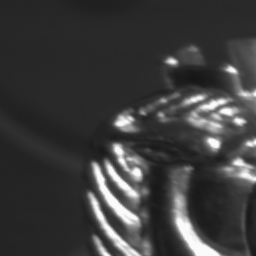
\includegraphics[width=0.34\linewidth]{100-clean.png}
%     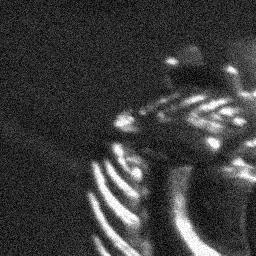
\includegraphics[width=0.34\linewidth]{100-noisy-mse.png}
%     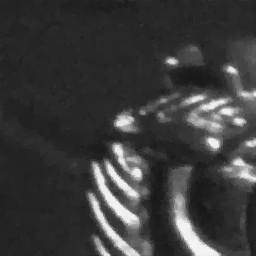
\includegraphics[width=0.34\linewidth]{100-psnr_34.02-lambda_0.04.png}
%     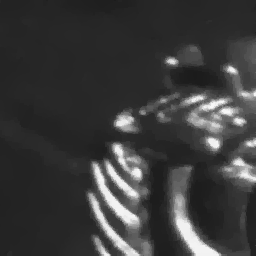
\includegraphics[width=0.34\linewidth]{100-denoised-mse_24.42-psnr_34.29-ssim_0.96.png}
%     \caption{SIDD example: Clean, Noisy, $\lambda = 0.04$ with PSNR = 34.02, $\mathbf{\Lambda}_\Theta$ with PSNR = 34.29}
%     \label{fig:SIDD-chest-example-1}
% \end{figure}

% \section{Acknowledgements}

% I would like to thank my supervisor, Dr. Kostas Papafitsoros, for his guidance and support throughout this project.

% I would like to thank at this point all the people that made this journey towards
% the completion of this Ph.D. thesis a pleasant one and made the last four years
% truly memorable.
% Firstly, I would like to thank Carola Sch¨onlieb for being an excellent supervisor
% from every perspective. Her continuous help and encouragement played a
% great role to my academic evolution. She was the one that introduced me to
% the field of mathematical imaging and showed me how a modern professional
% mathematician should be.
% The people I lived with in Cambridge played an important role during my
% Ph.D.. A big thanks goes to Sara Merino for being the best flatmate and
% friend possible for the last four years. The same amount of gratitude goes as
% well to Nayia Constantinou and Luca Calatroni. I could not have asked for
% better flatmates and good friends.
% A stimulating environment in the office makes the working hours pleasant
% and never boring. Bati Sengul and Spencer Hughes were an excellent pair of
% officemates and friends and I thank them a lot for that.
% I would like to thank Thalia Sotirchou for her love and support during the
% demanding last year of the Ph.D..
% Many thanks to all my friends in CCA and CMS, Marc Briant, Kolyan Ray
% (my gym-mate), Damon Civin, Ed Mottram, Vaggelis Papoutsellis, Julio Brau,
% Ioan Manolescu and also Panagiotis Kosteletos for all the nice moments we had
% together.
% Moreover, I would like to thank my collaborators Jan Lellmann, Kristian
% Bredies and Daniel Spector as well as Martin Benning and Tuomo Valkonen
% for useful discussions.
% I am grateful to the CCA directors Arieh Iserles and James Norris for giving me
% the opportunity to be part of it and to Emma Hacking for providing excellent
% administrative support. I also acknowledge the financial support provided
% by the Engineering and Physical Sciences Research Council, the Cambridge
% Centre for Analysis, the department of Pure Mathematics and Mathematical
% Statistics, the department of Applied Mathematics and Theoretical Physics
% and the King Abdullah University of Science and Technology.
% I would like to thank the thesis examiners Dr. Anders Hansen and Professor
% Antonin Chambolle for carefully reading the manuscript and for the fruitful
% discussion during the examination.
% Above all I would like to thank my mother Emmy, my sister Nassia and all my
% family, without whom I would not have achieved all these!


\section{Introduction}

- Rewrite parts written by ChatGPT, or written specifically for mini project but not relevant anymore

- Check consistent notations

- Redraw U-Net diagram

- Arrange figures in correct locations

% \subsection{Background}

% \begin{abstract}


In this dissertation we will describe the theory and application of the total variational (TV) method to image denoising. 
We will also describe the implementation of the method and an improvement using a U-Net architecture to find the regularisation parameters more efficiently. 
% We will then present the results of the method on a few different datasets.


Image processing, and image denoising in particular, has seen significant advancements since the U-Net was first applied in 2015. This project aims to build upon these advancements by implementing and experimenting with a U-Net-based model for image denoising.
% The paper \cite{kofler2023learning} that this project is based on discusses
In particular, it combines U-Net with a traditional image-denoising algorithm called the Primal Dual Hybrid Gradient (PDHG) algorithm \cite{kofler2023learning}.
% to solve the image denoising task. 
% While the specifics of the algorithm are outside the scope of this project, 
% the main idea is to use U-Net to learn the required input, so-called the regularisation parameters, of a specific image for the PDHG algorithm. 
Specifically, a PDHG solver is appended to the end of the U-Net, treating the solver as the final layer of the entire network to create an end-to-end unsupervised model.
% To denoise images, the PDHG algorithm requires defining some regularisation parameters as part of the cost function. 

% By treating PDHG as the final layer, this approach demonstrates the flexibility of neural networks and helps reduce the black-box nature of the network.

One notable aspect of using U-Net in this problem is that, instead of acting as a black box and outputting a denoised version of each input image, it outputs a parameter map used in another algorithm, demonstrating the flexibility of neural networks.
% This has two main advantages. Firstly, by learning the features that can be fed into a well-understood classic algorithm, 
% This approach demonstrates the flexibility of neural networks and helps reduce the black-box nature of the network. 

% Additionally, this approach helps solving the boundary problem when combining multiple patches of an image. Due to insufficient GPU memory, high-definition images must be downscaled or divided into patches for training, and combining patches in a black-box approach is challenging due to boundary issues. However, this approach combines patches of the regularisation parameter map, which can then be passed whole to the PDHG algorithm. The output of the PDHG algorithm typically does not show patch boundaries, resulting in smoother images.


% \end{abstract}


% \section{Overview}

% \section{Mathematical preliminaries}


% \subsubsection{What is image denoising?}

% \subsubsection{Why is image denoising important?}


% This project is largely based on the research paper "Learning regularisation Parameter-Maps for Variational Image Reconstruction using Deep Neural Networks and Algorithm Unrolling" \cite{kofler2023learning} and utilises part of the Smartphone Image Denoising Dataset (SIDD) \cite{SIDD_2018_CVPR}.

 
% I find image processing in general and image denoising in particular very interesting.

% The primary goal of this mini-project is to learn about a specific type of neural network called the U-Net, a convolutional network architecture
% designed for segmentation of images \cite{ronneberger2015unet}, and apply it to the problem of image denoising. 

% In the rest of this report, I will explain the task of learning a regularisation parameter map using U-Net, describe the U-Net architecture in this problem, discuss the modelling and training process, and finally present some preliminary results. 







% In this project, the model is trained and evaluated using the peak signal-to-noise ratio (PSNR) metric, and preliminary results are analysed to validate the approach. Additionally, the project adapts the code from the original paper, which was used for dynamic image denoising, to apply to static image denoising. This adaptation involved a complete rewriting, simplifying the code from over 200 lines to under 80 lines, making it more understandable and easier to modify. This simplification enabled further modifications, such as adding more layers to the network.

% Although much of the logic described in this project is implemented in an open-source project \cite{kofler2023learning}, getting started can be challenging. Therefore, a self-contained notebook with code and instructions to obtain the data was prepared to help fellow students experiment more easily. This notebook can run on Google Colab \cite{colab} and Kaggle \cite{kaggle}, providing an accessible platform for experimentation. Additionally, part of this report could serve as documentation for the open-source project, enhancing it with additional visualisations and explanations not provided in the original project. These additions aim to help readers of the paper gain a better understanding of the approach.



% \subsection{Denoising problems}

% The history of image denoising: 

% Image denoising began in the 1960s with the development of the Wiener filter, which is a linear filter that minimises the mean squared error between the denoised image and the original image.
% The Wiener filter works by finding the image that minimises the following objective function:

% \[
% \min_{I} \frac{1}{2} ||I - I_{\text{noisy}}||^2
% \]

% where $I$ is the denoised image, $I_{\text{noisy}}$ is the noisy image, and $||\cdot||$ is the mean squared error between two images.

% The Wiener filter is a linear filter that works well for images that are corrupted by Gaussian noise.
% However, the Wiener filter does not work well for images that are corrupted by non-Gaussian noise, such as salt-and-pepper noise.

% Before the advance of Neural networks, the total variational (TV) method was one of the most popular methods for image denoising.
% Total variational (TV) method is one of the most popular methods for image denoising.
% The TV method works by finding the image that has the smallest total variation and is closest to the noisy image in terms of the mean squared error.

% The TV method is based on the idea that images that are smooth have a small total variation, while images that are noisy have a large total variation.
% By minimising the total variation of the image, the TV method is able to remove the noise from the image and produce a smoother image \cite{RUDIN1992259}.

% The TV method is able to denoise images that are corrupted by non-Gaussian noise, such as salt-and-pepper noise, and is able to produce high-quality denoised images \cite{rudin1992nonlinear}.

% Before the advance of neural networks, image denoising was done by hand-crafted methods such as the total variational (TV) method \cite{rudin1992nonlinear}.

% Since the arrival of neural networks, the U-Net has been the most popular method for image denoising.

% The U-Net is a type of neural network that is commonly used for image segmentation.
% The U-Net is made up of a series of convolutional layers that downsample the image and a series of transposed convolutional layers that upsample the image.
% The U-Net is able to learn to segment images by training on a large dataset of images and their corresponding segmentation masks.

% The U-Net is able to learn to denoise images by training on a large dataset of noisy images and their corresponding clean images \cite{ronneberger2015unet}.

% The U-Net is able to produce high-quality denoised images that are close to the ground truth images \cite{ronneberger2015unet}.

Here we combine the traditional TV method with the U-Net to produce a more efficient method for image denoising.





\subsection{Total Variational Denoising}

The total variational (TV) method is a method for image denoising that is based on the principle of minimising the total variation of the image.
The total variation of an image is a measure of the amount of variation in the intensity of the image.
The TV method works by finding the image that has the smallest total variation and is closest to the noisy image in terms of the mean squared error.

The TV method is based on the idea that images that are smooth have a small total variation, while images that are noisy have a large total variation.
By minimising the total variation of the image, the TV method is able to remove the noise from the image and produce a smoother image.

% For a image $I \in \mathbb{R}^{w \times h}$,  $w, h \in \mathbb{N}$, we can represent the matrix $I$ with a vector $\mathbf{x} \in \mathbb{R}^n$ where $n = w \times h$.

Denoising problems can be described as 

\begin{equation}
  \mathbf{z} = \mathbf{x}_{\text{true}} + \mathbf{e}
\end{equation}
  
where $\mathbf{x}_{\text{true}} \in \mathbb{R}^{m \times n}$ is 
the object to be imaged, 
% the "true"/"clean" image,
% denoised image
$\mathbf{e} \in \mathbb{R}^{m \times n}$ denotes some random noise component, and $\mathbf{z} \in \mathbb{R}^{m \times n}$ represents 
the measured data.
% the noisy image.
The goal is to recover $\mathbf{x}_{\text{true}}$ or at least a good enough reconstruction given $\mathbf{z}$.

A prominent approach is to formulate the reconstruction as a minimisation problem:

% The total variational denoising method works by finding the image that minimises the following objective function:

\begin{equation}
  % \mathbf{x}_{\text{denoised}} = \arg \min_{\mathbf{x}} d(\mathbf{x}, \mathbf{z}) + \mathcal{R}(\mathbf{x})
  \hat{\mathbf{x}} = \arg \min_{\mathbf{x}} d(\mathbf{x}, \mathbf{z}) + \mathcal{R}(\mathbf{x})
\end{equation}

where $d(\cdot, \cdot)$ is a data fidelity term and $\mathcal{R}(\cdot)$ is a regularisation term.


Here we will look at Gaussian noise. The data fidelity term appropriate for Gaussian noise is the square of the $\ell_2$ norm:

\begin{equation}
  d(\mathbf{x}, \mathbf{z}) = \frac{1}{2} \|\mathbf{x} - \mathbf{z}\|_2^2
\end{equation}

The regularisation term $\mathcal{R}(\cdot)$ is the total variation of the image, which is a measure of the amount of variation in the intensity of the image. The total variation of an image can be calculated using the following formula:

\begin{equation}
  \mathcal{R}(\mathbf{x}) = \lambda \| \nabla \mathbf{x} \|_1
\end{equation}

where $\nabla \mathbf{x}$ is the gradient of the image $\mathbf{x}$ and $\lambda \in \mathbb{R}^{+}$ is a regularisation parameter that controls the trade-off between the total variation of the image and the mean squared error between the denoised image $\mathbf{x}$ and the noisy image $\mathbf{z}$.



$\nabla$ denotes a finite-differences operator.
% \cite{finite_difference_op}.
Finite difference operators include, forward difference operator,
backward difference operator, shift operator, central difference operator and mean operator.
% (\url{https://en.wikipedia.org/wiki/Total_variation_denoising#2D_signal_images})
Let us focus on the forward difference operator. In particular, in the discrete case, given a matrix $\mathbf{x}$, $\nabla \mathbf{x}$ is two matrices, one for the vertical gradient $\nabla_{x} \mathbf{x}$ and one for the horizontal gradient $\nabla_{y} \mathbf{x}$.

% This is the discrete case, and $\nabla \mathbf{x}$ can be the calculated in four different ways: forward, backward, central, and double-central (Sobel?). 

\begin{equation}
  \nabla \mathbf{x} = \begin{bmatrix}
    \nabla_{x} \mathbf{x} \\
    \nabla_{y} \mathbf{x}
  \end{bmatrix}
\end{equation}



For the forward gradient, the vertical gradient is calculated as:

\begin{equation}
  \begin{aligned}
  \nabla_{x} \mathbf{x} &= \begin{bmatrix}
    \mathbf{x}_{2,1} - \mathbf{x}_{1,1} & \mathbf{x}_{2, 2} - \mathbf{x}_{1, 2} & \ldots & \mathbf{x}_{2, n-1} - \mathbf{x}_{1, n-1} & \mathbf{x}_{2, n} - \mathbf{x}_{1, n} \\
    \mathbf{x}_{3,1} - \mathbf{x}_{2,1} & \mathbf{x}_{3, 2} - \mathbf{x}_{2, 2} & \ldots & \mathbf{x}_{3, n-1} - \mathbf{x}_{2, n-1} & \mathbf{x}_{3, n} - \mathbf{x}_{2, n}  \\
    \vdots & \vdots & \ddots & \vdots & \vdots \\
    \mathbf{x}_{m,1} - \mathbf{x}_{m-1,1} & \mathbf{x}_{m, 2} - \mathbf{x}_{m-1, 2} & \ldots & \mathbf{x}_{m, n-1} - \mathbf{x}_{m-1, n-1} & \mathbf{x}_{m, n} - \mathbf{x}_{m-1, n} \\
    \mathbf{x}_{1, 1} - \mathbf{x}_{m, 1} & \mathbf{x}_{1, 2} - \mathbf{x}_{m, 2} & \ldots & \mathbf{x}_{1, n-1} - \mathbf{x}_{m, n-1} & \mathbf{x}_{1, n} - \mathbf{x}_{m, n} \\
  \end{bmatrix} \\
  &= \begin{bmatrix}
    -1 & 1 & \ldots & 0 & 0 \\
    0 & -1 & \ldots & 0 & 0 \\
     \vdots & \vdots & \ddots & \vdots & \vdots \\
    0 & 0 & \ldots & -1 & 1 \\
    1 & 0 & \ldots & 0 & -1
    \end{bmatrix} \mathbf{x}
  \end{aligned}
\end{equation}

and the horizontal gradient is calculated as:

\begin{equation}
  \begin{aligned}
  \nabla_{y} \mathbf{x} &= \begin{bmatrix}
    \mathbf{x}_{1,2} - \mathbf{x}_{1,1} & \mathbf{x}_{1,3} - \mathbf{x}_{1,2} & \ldots & \mathbf{x}_{1,n} - \mathbf{x}_{1,n-1} & \mathbf{x}_{1,1} - \mathbf{x}_{1,n} \\
    \mathbf{x}_{2,2} - \mathbf{x}_{2,1} & \mathbf{x}_{2,3} - \mathbf{x}_{2,2} & \ldots & \mathbf{x}_{2,n} - \mathbf{x}_{2,n-1} & \mathbf{x}_{2,1} - \mathbf{x}_{2,n}  \\
    \vdots & \vdots & \ddots & \vdots & \vdots \\
    \mathbf{x}_{m-1,2} - \mathbf{x}_{m-1,1} & \mathbf{x}_{m-1,3} - \mathbf{x}_{m-1,2} & \ldots & \mathbf{x}_{m-1,n} - \mathbf{x}_{m-1,n-1} & \mathbf{x}_{m-1,1} - \mathbf{x}_{m-1,n} \\
    \mathbf{x}_{m,2} - \mathbf{x}_{m,1} & \mathbf{x}_{m,3} - \mathbf{x}_{m,2} & \ldots & \mathbf{x}_{m,n} - \mathbf{x}_{m,n-1} & \mathbf{x}_{m,1} - \mathbf{x}_{m,n} \\
  \end{bmatrix} \\
  &=  \mathbf{x} \begin{bmatrix}
    -1 & 0 & \ldots & 0 & 1 \\
    1 & -1 & \ldots & 0 & 0 \\
    \vdots & \vdots & \ddots & \vdots & \vdots \\
    0 & 0 & \ldots & -1 & 0 \\
    0 & 0 & \ldots & 1 & -1
    \end{bmatrix}
  \end{aligned}
\end{equation}



% \begin{equation}
%   \nabla \mathbf{x} = \left( \frac{\partial \mathbf{x}}{\partial x}, \frac{\partial \mathbf{x}}{\partial y} \right)
% \end{equation}


% Let

% \begin{equation}
% \nabla \mathbf{x} = \left( \frac{\partial \mathbf{x}}{\partial x_1}, \frac{\partial \mathbf{x}}{\partial x_2}, \ldots, \frac{\partial \mathbf{x}}{\partial x_n} \right)
% \end{equation}

% be the gradient of the image $\mathbf{x}$.
% $\nabla \mathbf{x}$ is a vector of partial derivatives of $\mathbf{x}$ with respect to each variable. Each component of $\nabla \mathbf{x}$ is the partial derivative of the corresponding component of $\mathbf{x}$ with respect to the corresponding variable.

We calculate the gradient in the horizontal and vertical directions separately, and then combine them to get the total variation of the image. 

\begin{equation}
  \| \nabla \mathbf{x} \|_1 = \| \nabla_x \mathbf{x} \|_1 + \| \nabla_y \mathbf{x} \|_1
\end{equation}

% \begin{equation}
%   TV(\mathbf{x}) = \|\nabla \mathbf{x}\|_1 = \sum_{z \in \mathcal{I}} \|\nabla \mathbf{x}(z)\|_1 := \sum_{z \in \mathcal{I}} \left( |\nabla_x \mathbf{x}(z)| + |\nabla_y \mathbf{x}(z)| \right),
% \end{equation}


% It is more convenient to use the notation $I$ to represent the image as a matrix so we can define the gradient.

For the forward gradient, the norm-1 of the vertical gradient is calculated as:

\begin{equation}
  \| \nabla_x \mathbf{x} \|_1 = \left( \sum_{i=1}^{m-1} \sum_{j=1}^{n} |\mathbf{x}_{i+1,j} - \mathbf{x}_{i,j}| \right) + \sum_{j=1}^{n} |\mathbf{x}_{1, j} - \mathbf{x}_{m,j}|
\end{equation}

and norm-1 of the horizontal gradient is calculated as:

\begin{equation}
  \| \nabla_y \mathbf{x} \|_1 = \left( \sum_{i=1}^{m} \sum_{j=1}^{n-1} |\mathbf{x}_{i,j+1} - \mathbf{x}_{i,j}| \right) + \sum_{i=1}^{m} |\mathbf{x}_{i, 1} - \mathbf{x}_{i,n}|
\end{equation}

% \begin{equation}
%   \| \nabla \mathbf{x} \|_1 = \text{TV}(I) = \sum_{i,j} |I_{i,j} - I_{i+1,j}| + |I_{i,j} - I_{i,j+1}|
% \end{equation}

% where $I_{i,j}$ is the intensity value of pixel $(i,j)$ in the image $I$. 
% % (Note: $I$ looks like the identity matrix. Is there a better notation?)

% \begin{equation}
%   \| \nabla \mathbf{x} \|_1 = \sum_{i,j} |\mathbf{x}_{i,j} - \mathbf{x}_{i+1,j}| + |\mathbf{x}_{i,j} - \mathbf{x}_{i,j+1}|
% \end{equation}

where $\mathbf{x}_{i,j}$ is the intensity value of pixel $(i,j)$ in the image $\mathbf{x}$. Note that $\mathbf{x}_{i,j}$ can be a scalar for a black-and-white image or a vector of 3 values for a colour image.

Note that, we can move $\lambda$ inside the norm, so the regularisation term can be written as:

\begin{equation}
    \mathcal{R}(\mathbf{x}) 
    = \lambda \| \nabla \mathbf{x} \|_1 \\
    = \| \lambda \nabla \mathbf{x} \|_1 \\
    = \| \lambda \nabla_x \mathbf{x} \|_1 + \| \lambda \nabla_y \mathbf{x} \|_1
\end{equation}

% % Write a aligned equation
% \begin{equation}
%   \begin{aligned}
%     \mathcal{R}(\mathbf{x}) 
%     &= \lambda \| \nabla \mathbf{x} \|_1 \\
%     &= \| \lambda \nabla \mathbf{x} \|_1 \\
%     &= \text{TV}(\lambda I) \\
%     &= \sum_{i,j} |\lambda I_{i,j} - \lambda I_{i+1,j}| + |\lambda I_{i,j} - \lambda I_{i,j+1}|
%   \end{aligned}
% \end{equation}

The regularisation parameter does not need to be a scalar.
% Each pixel in the image can have its own regularisation parameter.
We can swap the scalar $\lambda$ with a regularisation parameter map $\mathbf{\Lambda}$,

\begin{equation}
  \mathbf{\Lambda} = \begin{bmatrix}
    \mathbf{\Lambda}^{(x)} \\
    \mathbf{\Lambda}^{(y)}
  \end{bmatrix}
\end{equation}

where $\mathbf{\Lambda}^{(x)}, \mathbf{\Lambda}^{(y)} \in \mathbb{R}^{m \times n}$ are matrices that contain the regularisation parameters for the vertical and horizontal gradients respectively.
Here we will assume $\mathbf{\Lambda}^{(x)} = \mathbf{\Lambda}^{(y)}$ and denote them as $\mathbf{\Lambda}^{(xy)}$, i.e.
\begin{equation}
  \mathbf{\Lambda} = \begin{bmatrix}
    \mathbf{\Lambda}^{(xy)} \\
    \mathbf{\Lambda}^{(xy)}
  \end{bmatrix}
\end{equation}

This gives us a new regularisation term that can be written as
% $\in \mathbb{R}^{m \times n}$, 
% where each element of $\mathbf{\Lambda}$ is a regularisation parameter for the corresponding pixel in the image $\mathbf{x}$.



% $\lambda$, but can be a diagonal matrix $\mathbf{\Lambda} \in \mathbb{R}^{n}$.

\begin{equation}
  \mathcal{R}(\mathbf{x}) = \| \mathbf{\Lambda} \circ \nabla \mathbf{x} \|_1
  = \| \mathbf{\Lambda}^{(xy)} \circ \nabla_x \mathbf{x} \|_1 + \| \mathbf{\Lambda}^{(xy)} \circ \nabla_y \mathbf{x} \|_1
\end{equation}

where $\circ$ denotes the Hadamard or element-wise product.
% We will refer to $\mathbf{\Lambda}$ as the regularisation parameter map.



Putting it all together, 
% the total variation of an image 
the solution to the total variational denoising problem
can be 
% calculated
defined
using the following formula:

\begin{equation}
  % \mathbf{x}_{\text{denoised}} = \arg \min_{\mathbf{x}} \frac{1}{2} \|\mathbf{x} - \mathbf{z}\|_2^2 + \lambda \| \nabla \mathbf{x} \|_1
  \hat{\mathbf{x}} = \arg \min_{\mathbf{x}} \frac{1}{2} \|\mathbf{x} - \mathbf{z}\|_2^2 + \lambda \| \nabla \mathbf{x} \|_1
\end{equation}

if we use a scalar $\lambda$ regularisation parameter, or

\begin{equation} \label{eq:1}
  \hat{\mathbf{x}} = \arg \min_{\mathbf{x}} \frac{1}{2} \|\mathbf{x} - \mathbf{z}\|_2^2 + \| \mathbf{\Lambda} \circ \nabla \mathbf{x} \|_1
\end{equation}

if we use a regularisation parameter map $\mathbf{\Lambda}$ of regularisation parameters.

In this dissertation, we will use
U-Net to help us find the regularisation parameter map $\mathbf{\Lambda}$ 
% that the later form of the regularisation term.
% The U-Net will be used to find the regularisation parameter map $\mathbf{\Lambda}$ 
given any (noisy) image. 
We will compare the results to the best-case scenario where we use a scalar regularisation parameter $\lambda$.

% Question: Idealy, if we pass in a clean image to U-Net then all the regularisation parameters should be zero, right?


% The total variational denoising method works by finding the image that has the smallest total variation and is closest to the noisy image in terms of the mean squared error.
% The total variation of an image is defined as the sum of the absolute differences between the intensity values of neighbouring pixels.


% where $\lambda$ is a regularisation parameter that controls the trade-off between the total variation of the image and the mean squared error between the denoised image $I$ and the noisy image $I_{\text{noisy}}$.

\subsection{U-Net}

The U-Net is a type of neural network that is commonly used for image segmentation \cite{ronneberger2015unet}.
The U-Net is an encoder-decoder network that is designed to take an image as input and produce a segmentation mask as output.
The U-Net is made up of a series of convolutional layers that downsample the image and a series of transposed convolutional layers that upsample the image.
The U-Net is able to learn to segment images by training on a large dataset of images and their corresponding segmentation masks.

We refer to the set of trainable parameters in the U-Net as $\Theta$, and the output of the U-Net as $\Lambda_{\Theta}$.

In our case, we will optimise a U-Net model to find the regularisation parameter map $\Lambda_{\Theta}$ that produces the best denoised image for any particular noisy image.


\subsection{Related Work}


\subsection{Contribution}

- Adapt the existing code of the dynamic image denoising project in \cite{kofler2023learning} to static image denoising. Train and evaluate the model using a new dataset - Chest X-ray dataset.

- Present the theory of the total variational denoising method and the experimental set-up in detail so that a fellow student can understand the method and implement it themselves.



% The U-Net is a type of neural network that is commonly used for image segmentation.
% The U-Net is made up of a series of convolutional layers that downsample the image and a series of transposed convolutional layers that upsample the image.
% The U-Net is able to learn to segment images by training on a large dataset of images and their corresponding segmentation masks.

% \begin{enumerate}
%     \item The noisy image was passed through a U-Net to produce an initial denoised image.
%     \item The total variation of the denoised image was calculated using the formula above.
%     \item The regularisation parameter $\lambda$ was found by minimising the following objective function:
    
%     \[
%     \min_{\lambda} \lambda TV(I) + \frac{1}{2} ||I - I_{\text{noisy}}||^2
%     \]
    
%     \item The denoised image was then found by minimising the following objective function:
    
%     \[
%     \min_{I} \lambda TV(I) + \frac{1}{2} ||I - I_{\text{noisy}}||^2
%     \]
% \end{enumerate}




\section{Method and Implementation}



\subsection{Primal Dual Hybrid Gradient (PDHG)}

To solve equation
(14) 
% \ref{eq:1}, 
we can use an iterative method called the Primal Dual Hybrid Gradient (PDHG). 

The algorithm is

\begin{algorithm}[H]
\caption{PDHG algorithm for image denoising with fixed regularization parameter-map $\boldsymbol{\Lambda}$ (adapted from ...)}
\begin{algorithmic}[1]
\STATE \textbf{Input:} $L = \| [\mathbf{I}, \nabla]^\text{T} \|$, $\tau = 1/L$, $\sigma = 1/L$, $\theta = 1$, noisy image $\mathbf{x}_0$
\STATE \textbf{Output:} reconstructed image $\hat{\mathbf{x}}$
% \STATE $\mathbf{y} = \mathbf{x}_0$
\STATE $\bar{\mathbf{x}}_0 = \mathbf{x}_0$
\STATE $\mathbf{p}_0 = 0$
\STATE $\mathbf{q}_0 = 0$
\FOR{$k < T$}
    % \STATE $\mathbf{p}_{k+1} = \left(\mathbf{p}_k + \sigma ( \bar{\mathbf{x}}_k - \mathbf{y})\right) / (1 + \sigma)$
    \STATE $\mathbf{p}_{k+1} = \left(\mathbf{p}_k + \sigma ( \bar{\mathbf{x}}_k - \mathbf{x}_0)\right) / (1 + \sigma)$
    \STATE $\mathbf{q}_{k+1} = \text{clip}_{\boldsymbol{\Lambda}} \left(\mathbf{q}_k + \sigma \nabla \bar{\mathbf{x}}_k \right)$
    \STATE $\mathbf{x}_{k+1} = \mathbf{x}_k - \tau \mathbf{p}_{k+1} - \tau \nabla^\text{T} \mathbf{q}_{k+1}$
    \STATE $\bar{\mathbf{x}}_{k+1} = \mathbf{x}_{k+1} + \theta (\mathbf{x}_{k+1} - \mathbf{x}_k)$
\ENDFOR
\STATE $\hat{\mathbf{x}} = \mathbf{x}_T$
\end{algorithmic}
\end{algorithm}

where $\mathbf{I}$ is the identity matrix, $\text{clip}_{\boldsymbol{\Lambda}}$ is a function that clips the values of $\mathbf{q}_{k+1}$ to the range $[0, \boldsymbol{\Lambda}]$.

The choice of $L$ is taken from \cite{Sidky_2012} \url{https://iopscience.iop.org/article/10.1088/0031-9155/57/10/3065/pdf}. 
The number of iterations $T$ is a hyperparameter that we can choose for the training process.

(TODO: Understand what $L$ is. Do we need to include $\theta = 1$? Can we write $\bar{\mathbf{x}}_{k+1} = 2 \mathbf{x}_{k+1} - \mathbf{x}_k$? In the code, initially $\mathbf{p}_0 = \mathbf{x}_0$?)

% (For comparison with the original version in \cite{kofler2023learning}:

% 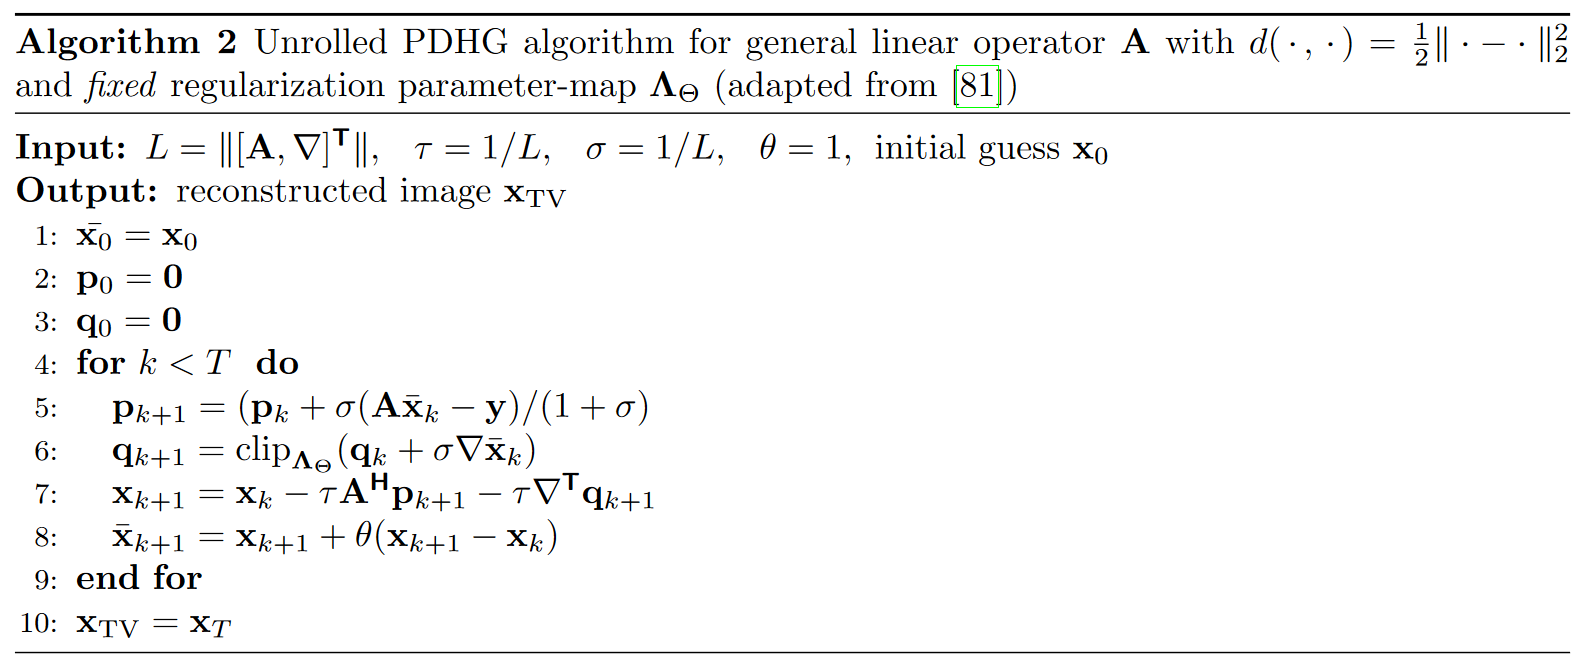
\includegraphics[width=1\linewidth]{images/references/PDHG original.png}

% For denoising, $\mathbf{A}$ is the identity matrix. If $\mathbf{A}^{\text{H}}$ is the conjugate transpose, then it is also an identity matrix.)

% NOTE: $\mathbf{y}$ is the noisy image $\mathbf{x}_0$ ???

% HOWEVER, note that in the code, $\mathbf{p}_{k+1} = \left(\mathbf{p}_k + \sigma  \times (\bar{\mathbf{x}}_k - \mathbf{y})\right) / (1 + \sigma)$

% \subsection{Objective}


% % Traditionally, the Total Variation (TV) method has been used to improve image reconstruction \cite{kofler2023learning}. 
% % For this method to work effectively, we need to learn the optimal regularisation parameters.
% One of the most widely applied image denoising methods is the so-called Total Variation (TV) regularisation \cite{kofler2023learning}.

% Formally, given the loss function
% \vspace{-3pt}
% $$ L(\mathbf{z}, \mathbf{x}) = \frac{1}{2} \| \mathbf{x} - \mathbf{z} \|_2^2 + \text{TV}(\mathbf{x}), $$

% our objective is to find $\hat{\mathbf{x}}$ such that
% $$ \hat{\mathbf{x}} = \arg \min_{\mathbf{x}} L(\mathbf{z}, \mathbf{x}) $$
% where $\mathbf{z}$ is the input, presumably noisy, image and $\mathbf{x}$ represent the "clean" image we are looking for. We treat images as vectors, $\mathbf{x}, \mathbf{z} \in \mathbb{R}^{n^2}$, where $n$ is the height of the image, assuming the image is square. In this project, we use $n = 512$.

%  The $\text{TV}$ term can be expressed as either a scalar $\lambda$:
% $$
% \text{TV}(\mathbf{x}) = \lambda \| \nabla \mathbf{x} \|_1, \quad \lambda \in \mathbb{R}
% $$
% or as a matrix $\mathbf{\Lambda}$:
% $$
% \text{TV}(\mathbf{x}) = \| \mathbf{\Lambda} \nabla \mathbf{x} \|_1, \quad \mathbf{\Lambda} \in \mathbb{R}^{n^2}
% $$

% Here, $\nabla \mathbf{x}$ represents the spatial gradient, i.e., the difference between adjacent pixels. We use the forward gradient, which calculates the difference between the current pixel and the pixels in the next row and next column.


The problem with TV method is that it is not clear how to choose the regularisation parameter $\lambda$.
The U-Net can be used to find the regularisation parameter $\lambda$ more efficiently.
After training with many examples, the U-Net can learn to predict the regularisation parameter $\lambda$ that produces the best denoised image for any particular noisy image.


The challenge lies in finding or learning the regularisation parameter map $\mathbf{\Lambda}$. Using a single $\lambda$ value penalises all regions of the image equally, which is suboptimal. Instead, it would be better to assign higher penalties to smooth regions and lower penalties to detailed regions to preserve image details. However, this approach is not perfect, as it might leave noise in detailed areas.

Since regularisation is multiplied by the gradient, higher $\lambda$ values will penalize areas with many changes (typically areas with more details), while lower $\lambda$ values prioritize detail preservation over noise reduction.

The performance of Primal-Dual Hybrid Gradient (PDHG) methods can be improved by assigning suitable regularisation parameters to regions based on their characteristics. However, narrowing down the search space is challenging, as we potentially have $d^{(n^2)}$ different maps to consider, where $d$ is the number of $\lambda$ values (typically around 100, ranging from 0.01 to 1) and $n$ is the image dimension. This is computationally infeasible.

To address this, we can apply image segmentation. Effective image segmentation helps determine appropriate $\lambda$ values for different regions. A good network for learning image segmentation is U-Net \cite{ronneberger2015unet}.

% U-Net assists in learning these regularisation parameters due to its proficiency in image segmentation. 


\section{Architecture}

\begin{figure}[ht]
    \centering
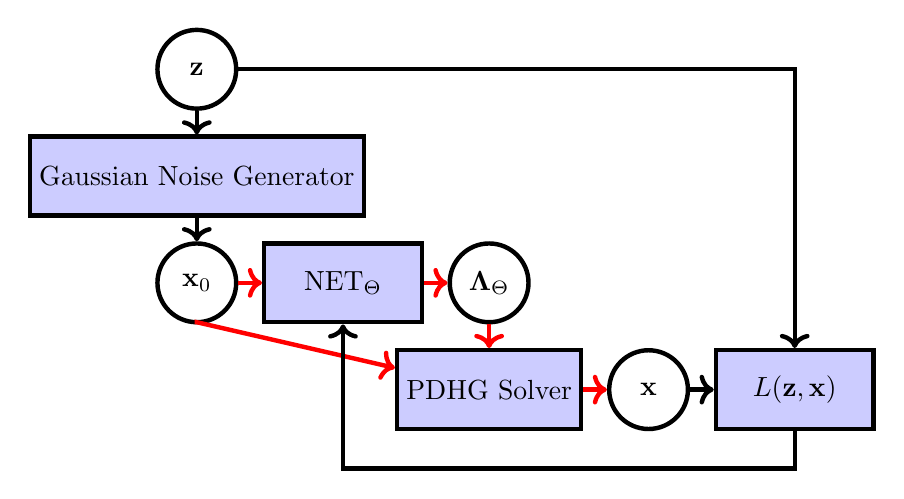
\begin{tikzpicture}[node distance=0.3cm, auto, ultra thick]

    % Define styles for the different layers
    \tikzstyle{output} = [draw, circle, minimum width=1cm, minimum height=1cm]
    \tikzstyle{function} = [draw, rectangle, minimum width=2cm, minimum height=1cm, fill=blue!20]
    \tikzstyle{inference} = [->, ultra thick, red]
    \tikzstyle{normal} = [->, ultra thick, black]

    \node (input) [output] {$\mathbf{x}_0$};
    \node (unet) [function, right=of input] {$\text{NET}_{\Theta}$};
    \node (lambda) [output, right=of unet] {$\mathbf{\Lambda}_{\Theta}$};
    \node (pdhg) [function, below=of lambda] {PDHG Solver};
    \node (final_output) [output, right=of pdhg] {$\mathbf{x}$};   
    \node (noise_generator) [function, above=of input] {Gaussian Noise Generator};
    \node (ground_truth) [output, above=of noise_generator] {$\mathbf{z}$};
    \node (loss_function) [function, right=of final_output] {$L(\mathbf{z}, \mathbf{x})$};

    \draw[inference] (input) -- (unet);
    \draw[inference] (unet) -- (lambda);
    \draw[inference] (lambda) -- (pdhg);
    \draw[inference] (pdhg) -- (final_output);
    \draw[inference] (input) -- ++(0, -0.5) -- (pdhg);
    
    \draw[->] (final_output) -- (loss_function);
    \draw[->] (ground_truth) -| (loss_function);
    \draw[->] (ground_truth) -- (noise_generator);
    \draw[->] (noise_generator) -- (input);
    \draw[->] (loss_function) -- ++(0, -1) -| (unet);

\end{tikzpicture}

\caption{The general architecture 
% \caption{Training 
% of PDHG Net 
% \cite{kofler2023learning}
}

\label{fig:training}
\end{figure}



For this project, our model comprises two primary components:
\begin{enumerate}
    \item A U-Net, denoted as $\text{NET}_{\Theta}$, which is responsible for learning the regularisation parameters $\mathbf{\Lambda}_{\Theta}$ from an input image $\mathbf{x}_0$.
    \item A Primal Dual Hybrid Gradient (PDHG) algorithm solver (refer to Appendix), which utilizes both $\mathbf{z}$ and $\mathbf{\Lambda}_{\Theta}$ to transform $\mathbf{x}_0$ into $\hat{\mathbf{x}}$. This transformation aims to minimise the loss function $L(\mathbf{z}, \mathbf{x})$, thereby facilitating effective reconstruction. The symbol $\Theta$ represents the set of trainable parameters within the network.
\end{enumerate}

We interpret the PDHG solver as the ultimate hidden layer within our network. The outcome of the loss function $L(\mathbf{z}, \mathbf{x})$ is subsequently employed for backpropagation, essential for training the parameters $\Theta$.

For our implementation, we consider $n \times n$ images, specifically with $n = 512$.

In terms of variables:
\begin{itemize}
    \item $\mathbf{z} \in \mathbb{R}^{n^2}$ represents the clean image, serving as the ground truth.
    \item $\mathbf{x}_0 \in \mathbb{R}^{n^2}$ denotes the noisy image inputted to $\text{NET}_{\Theta}$.
    \item $\mathbf{\Lambda}_{\Theta}$, the regularisation parameters map, emerges as the final output from the U-Net and is instrumental for the PDHG algorithm solver. Throughout this project, $\mathbf{\Lambda}$ and $\mathbf{\Lambda}_{\Theta}$ are used interchangeably.
\end{itemize}

The architecture of $\text{NET}_{\Theta}$ is inspired by the U-Net, a specialised type of convolutional neural network architecture.

Let us first delve into the foundational concept of a convolutional neural network, which underpins the U-Net architecture.



\subsection{
Convolutional Neural Network (CNN) 
}

\begin{figure}[ht]
    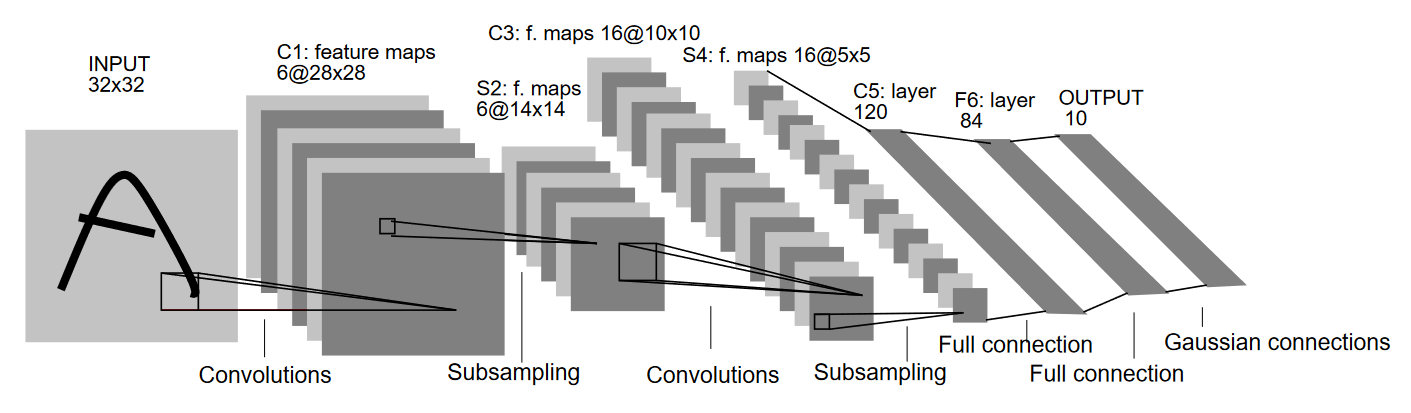
\includegraphics[width=1\linewidth]{Le-Net 5.png}
    
    \caption{Architecture of LeNet-5, one of the earliest Convolutional Neural Networks \cite{726791}} 
    \label{fig:enter-label}
\end{figure}

Convolutional Neural Networks (CNNs) are specialised types of artificial neural networks optimised for analyzing image data and other grid-like structures. We base our understanding on a two-dimensional (2D) CNN architecture, where each layer is comprised of one or more 2D matrices, in contrast to the vectors used in standard "vanilla" neural networks.

\subsubsection*{Inspiration and Function}

The design of CNNs draws inspiration from the human visual cortex, which processes visual stimuli by sequentially extracting features, ranging from simple edges and shapes to complex objects. CNNs replicate this hierarchical feature extraction using convolutional layers and pooling layers. 

\subsubsection*{Convolutional Layers}

In a convolutional layer, each output element results from a linear combination of inputs, processed through an activation function—akin to "vanilla" neural networks. However, the critical difference lies in the utilization of filters (or kernels). Each filter traverses the input matrix, computes the dot product with the corresponding input elements, and channels the result through an activation function. 
A single filter generates one output matrix, termed a feature map, acting as a feature extractor that emphasizes specific characteristics of the input. 
When multiple filters are employed in a layer, they produce multiple feature maps, with each map corresponding to a different channel. 
This design significantly reduces the proportion of trainable parameters relative to the number of output values, enhancing efficiency for image-related tasks.

\subsubsection*{Pooling Layers}

An essential component of CNNs is the pooling layer, typically implemented as a max-pooling layer. This layer simplifies the output by retaining only the maximum values from the defined regions in the feature map. The objective is to preserve the most significant features while reducing data dimensionality. In this project, max-pooling is a crucial technique used to enhance model performance.

The convolutional and pooling layers constitute the foundational blocks of the U-Net architecture.

\subsection{U-Net}



A U-Net, as introduced by Ronneberger et al. \cite{ronneberger2015unet}, extends the conventional CNN architecture by incorporating skip connections, akin to those in a residual network. These skip connections concatenate the outputs of distinct convolutional layers to generate a larger composite output.

\subsubsection*{Encoder}

The U-Net architecture is divided into two principal components: an Encoder and a Decoder. The Encoder functions similarly to a standard CNN, utilizing a combination of convolutional layers and max-pooling layers organized into distinct "blocks." In this project, each Encoder block comprises a pair of convolutional layers followed by a max-pooling layer, designed to successively double the number of channels (or feature maps) while concurrently reducing the feature map size due to the pooling.

\subsubsection*{Decoder}

Conversely, the Decoder is structured around a series of blocks that progressively halve the number of channels while enlarging the feature map size, effectively "unrolling" the data. Unlike the Encoder blocks, each Decoder block concludes with an up-convolutional layer followed by a skip connection. This up-convolutional layer, essentially a regular convolutional layer, outputs data that is then concatenated with the output from a corresponding Encoder block, facilitating the feature integration across different layers of the network.


% The U-Net was implemented using the following architecture:

% \begin{enumerate}
%     \item The U-Net was made up of a series of convolutional layers that downsampled the image by a factor of 2.
%     \item The U-Net was made up of a series of transposed convolutional layers that upsampled the image by a factor of 2.
%     \item The U-Net was trained on a large dataset of images and their corresponding segmentation masks.
%     \item The U-Net was able to learn to segment images by training on the dataset.
%     \item The U-Net was able to produce segmentation masks that were close to the ground truth masks.
%     \item The U-Net was able to generalise to new images and produce accurate segmentation masks.
% \end{enumerate}


\begin{figure}[ht]
\hspace*{-0.5cm} % Adjust the value as needed
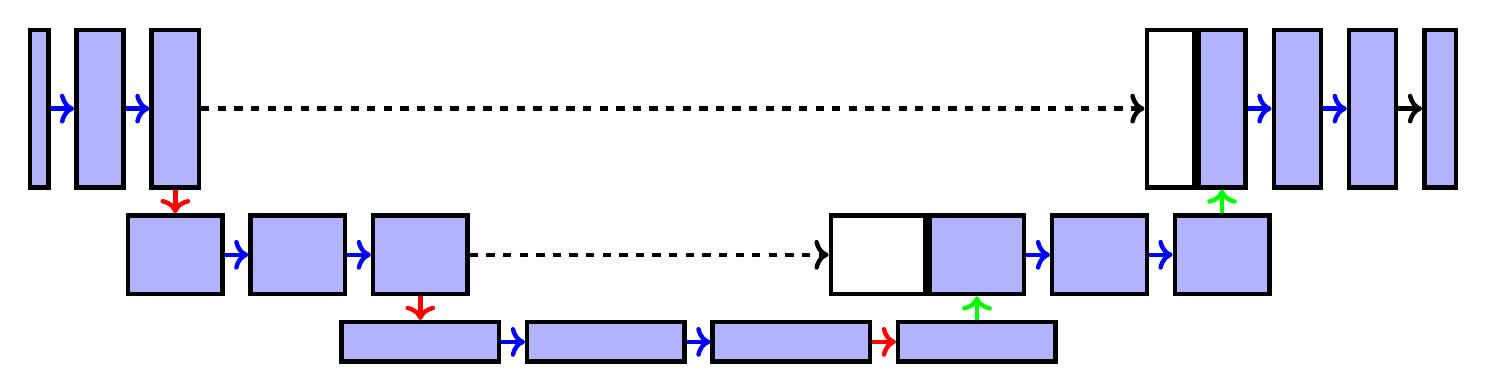
\begin{tikzpicture}[node distance=0.3cm, auto, ultra thick, transform shape, shift={(-10cm,0)}]
    % Define styles
    \tikzstyle{rec16_1} = [draw, rectangle, minimum width=0.1cm, minimum height=2cm, fill=blue!30]
    \tikzstyle{rec16} = [draw, rectangle, minimum width=0.6cm, minimum height=2cm, fill=blue!30]
    \tikzstyle{rec32} = [draw, rectangle, minimum width=1.2cm, minimum height=1cm, fill=blue!30]
    \tikzstyle{rec64} = [draw, rectangle, minimum width=2.0cm, minimum height=0.5cm, fill=blue!30]
    \tikzstyle{rec64_2} = [draw, rectangle, minimum width=2.0cm, minimum height=0.5cm, fill=blue!30]
    \tikzstyle{rec2} = [draw, rectangle, minimum width=0.4cm, minimum height=2cm, fill=blue!30]
    \tikzstyle{rec_white32} = [draw, rectangle, minimum width=1.2cm, minimum height=1cm, fill=white]
    \tikzstyle{rec_white16} = [draw, rectangle, minimum width=0.6cm, minimum height=2cm, fill=white]
    \tikzstyle{normalconv} = [->, ultra thick, blue]
    \tikzstyle{maxpool} = [->, ultra thick, red]
    \tikzstyle{upconv} = [->, ultra thick, green]
    \tikzstyle{finalconv} = [->, ultra thick, black]

    % ENCODER
    \node (en1_input) [rec16_1] {};
    \node (en1con1_output) [rec16, right=of en1_input] {};
    \node (en1con2_output) [rec16, right=of en1con1_output] {};

    \node (en2_input) [rec32, below=of en1con2_output] {};
    \node (en2con1_output) [rec32, right=of en2_input] {};
    \node (en2con2_output) [rec32, right=of en2con1_output] {};

    \node (en3_input) [rec64, below=of en2con2_output] {};
    \node (en3con1_output) [rec64, right=of en3_input] {};
    \node (en3con2_output) [rec64, right=of en3con1_output] {};
    \node (upcon1_input) [rec64_2, right=of en3con2_output] {};

    % DECODER
    \node (de1_input) [rec32, above=of upcon1_input] {};
    \node (skip1_output) [rec_white32, left=0cm of de1_input] {};
    \node (de1con1_output) [rec32, right=of de1_input] {};
    \node (de1con2_output) [rec32, right=of de1con1_output] {};

    \node (de2_input) [rec16, above=of de1con2_output] {};
    \node (skip2_output) [rec_white16, left=0cm of de2_input] {};
    \node (de2con1_output) [rec16, right=of de2_input] {};
    \node (de2con2_output) [rec16, right=of de2con1_output] {};

    % Final output layer
    \node (final_output) [rec2, right=of de2con2_output] {};

    % CONNECTIONS
    \draw[normalconv] (en1_input) -- (en1con1_output);
    \draw[normalconv] (en1con1_output) -- (en1con2_output);
    % \draw[maxpool] (en1con2_output) -- ++(0,-0.5) -| (en2_input);
    \draw[maxpool] (en1con2_output) -- (en2_input);
    
    \draw[normalconv] (en2_input) -- (en2con1_output);
    \draw[normalconv] (en2con1_output) -- (en2con2_output);
    % \draw[maxpool] (en2con2_output) -- ++(0,-0.5) -| (en3_input);
    \draw[maxpool] (en2con2_output) -- (en3_input);
    
    \draw[normalconv] (en3_input) -- (en3con1_output);
    \draw[normalconv] (en3con1_output) -- (en3con2_output);
    \draw[maxpool] (en3con2_output) -- (upcon1_input);
    
    % \draw[upconv] (en3con2_output) -- ++(0,0.5) -| (de1_input);
    \draw[upconv] (upcon1_input) -- (de1_input);
    \draw[normalconv] (de1_input) -- (de1con1_output);
    \draw[normalconv] (de1con1_output) -- (de1con2_output);
    
    % \draw[upconv] (de1con2_output) -- ++(0,0.5) -| (de2_input);
    \draw[upconv] (de1con2_output) -- (de2_input);
    \draw[normalconv] (de2_input) -- (de2con1_output);
    \draw[normalconv] (de2con1_output) -- (de2con2_output);
    
    \draw[finalconv] (de2con2_output) -- (final_output);

    % Skip connections
    \draw[->, dashed, ultra thick] (en2con2_output.east) -- ++(0.5,0) |- (skip1_output.west);
    \draw[->, dashed, ultra thick] (en1con2_output.east) -- ++(0.5,0) |- (skip2_output.west);

\end{tikzpicture}
\caption{Our $\text{NET}_{\Theta}$ Architecture}
\label{fig:my_unet}
\end{figure}

In our model, the Encoder consists of three encoding blocks. 
First we increase the number of channels to 32.
The first block the double the number of channels to 
64 feature maps. 
The second and third blocks increase the number of channels further to 128 and 256, respectively.

% Conversely, the Decoder incorporates two decoding blocks, one fewer than the Encoder. This configuration deviates from some common implementations where the number of encoding and decoding blocks are equal, and a "bottle-neck" comprising two additional convolutional layers is placed between them. In our model, we treat the final block of the Encoder as this bottle-neck. The first decoding block in the Decoder reduces the number of channels back to 32, and the second further reduces them to 16.

Similarly we have three decoding blocks.
Each decoding block in our model concludes with an up-convolutional layer, which serves the same function as a typical convolutional layer, followed by a skip connection. The first skip connection takes the 32-channel output from the second encoding block and merges it with the 32-channel output from the first up-convolutional layer. This combination produces a 64-channel output, which is then processed by the first decoding block. The second skip connection similarly merges the 16-channel output from the first encoding block with the 16-channel output from the second up-convolutional layer, resulting in a 32-channel input for the second decoding block.

The final stage in our architecture employs a convolutional layer to convert the 16-channel output from the last decoding block into a 2-channel output, thus producing two matrices as the ultimate output of our model.



\section{Experimental Set-Up}

% We used two datasets for the experiments: the Chest X-ray dataset and the SIDD dataset.

% \subsection{Chest X-ray Dataset}

We used the Chest X-Ray Images (Pneumonia) dataset which was downloaded from \url{https://www.kaggle.com/datasets/paultimothymooney/chest-xray-pneumonia}. 
This is a dataset for binary classification of normal and pneumonia chest X-ray images. 
The dataset consists of 5,863 X-Ray images (JPEG) and 2 categories (Pneumonia/Normal).
All images are black-and-white and are in the JPEG format.
The X-rays images have various resolutions.

At the time of download, the original dataset had already been split into a training set, a validation set, and a test set.
We picked 800 images for the training dataset for training and 100 images from the test set for testing. The validation set consists of only 8 images which were all used for validation.
We used only images which were classified as normal.

For consitent input, we cropped the images to squares and then resized them to $256 \times 256$.
For each image we generated a random value of $\sigma$ uniformly in the range from 0.1 to 0.5, and noised the image with Gaussian noise with mean 0 and the corresponding standard deviation $\sigma$.

% \subsection{SIDD Dataset}

% The original SIDD dataset consists of 320 images of various resolutions taken from the SIDD dataset \cite{sidd}.
% All images are sRGB and are in the PNG format.
% For each image, we randomly chose 32 patches of size 256x256 pixels.
% For each patch, we generated a random value of $\sigma$ ranging from 0.1 to 0.5 and noised the patch with Gaussian noise with that $\sigma$.
% We randomly picked 800 patches for the training dataset, 100 patches for the validation dataset, and 100 patches for the test dataset.

% \section{Experiments}

% We performed various experiments on the Chest X-ray dataset and the SIDD dataset with various configurations of the total variational denoising method and the U-Net.

% For both datasets, 
For learning the regularisation parameter map $\mathbf{\Lambda}_{\Theta}$, we used a U-Net structure with 1 initial double convolutional block, followed by 3 encoding blocks, 3 decoding blocks, and 1 final fully connected layer.
The number of initial filters, or output channels of the first convolution layer, is set to 32.
As commonly done, each encoding/decoding block contains a(n) downsampling/upsampling step, followed by 2 (fully) convolutional layers, in which the first convolutional layer doubles/halves the number channels which the second maintains the number of channels.
In other words, the number of output channels of each subsequent encoding block is doubled, while the number of output channels of each subsequent decoding block is halved.
The U-Net has 1 input channel and 2 final output channels.
This leads to a 1-32-64-128-256-128-64-32-2 structure.

All convolutional layers have a kernel size of $3 \times 3$ and a stride of 1.
Each side of a feature map has zero-padding of size 1 to maintain the size of the feature map after the convolution.
Keeping the number of size of the feature map constant after each convolution has the advantage of making the implementation of the skip connections simpler by not having to crop the output of the encoding blocks to match the size of the input of the decoding blocks.

Each encoding block begins with a max pooling layer with $2 \times 2$ kernels and a step size of 2.
Prior to the max pooling, a zeo-padding of size 1 is added in order to exactly halve the length of each side of the output.
On the other hand, all upsampling steps are done with linear interpolation with a scale factor of 2 which doubles the length of each side of the feature map.
In the end, the total number of trainable parameters of the set $\Theta$ is 1,796,034.

For the activation function, we used the Leaky ReLU with a negative slope of 0.01.
For the primal dual solver, we set the up-bound parameter to 0 and $T_{\text{train}}$ to 256.
During testing we also set $T_{\text{test}}$ to 256.

For reproducibility, we manually set a seed value to 42 for the random number generator at the beginning of the training process. We use the Adam optimiser with an initial learning rate of 1e-4, a batch size of 1, and the Mean Square Error (MSE) loss function. We trained for a total of 500 epochs.

It is worth noting that, for the implementation of the U-Net, 
we used the 3D implementations of the convolutional layers as well as the downsampling and upsmapling steps from the PyTorch library \cite{NEURIPS2019_9015}.
The main reasons we went with 3D instead of the 2D implementations are convenience and generality.
The 3D U-Net implementation is adapted from the dynamic image denoising application in \cite{kofler2023learning}, and can therefore be extended to 3D dynamic imaging applications in the future.

%     "in_channels": 1,
%     "out_channels": 2,
%     "init_filters": 32,
%     "n_blocks": 3,
%     "activation": "LeakyReLU",
%     "downsampling_kernel": (2, 2, 1),
%     "downsampling_mode": "max",
%     "upsampling_kernel": (2, 2, 1),
%     "upsampling_mode": "linear_interpolation",

%     "optimizer": "Adam",
%     "learning_rate": 1e-4,
%     "loss_function": "MSELoss",

%     "up_bound": 0,
    
%     "device": "cuda:0",

%     "wandb_mode": "online",
%     "save_epoch_wandb": 10_000,
%     "save_epoch_local": 10,
%     "save_dir": "tmp_2",




% \section{Results}

% Here we present the results for two datasets: the Chest X-ray dataset and the SIDD dataset.

% \subsection{Chest X-ray Dataset}

% The Chest X-ray dataset consists of 2000 images of chest X-rays of various resolutions. 
% All images are black-and-white and are in the JPEG format.
% I used 800 images for the training dataset, 100 images for the validation dataset, and 100 images for the test dataset.
% I used a U-Net with 3 blocks and 32 initial filters to denoise the images.

% All images were resized to 256x256 pixels and noised with Gaussian noise with $\sigma$ ranging from 0.1 to 0.5.





% \section{Experimental Set-up}



% \subsection{Chest X-ray}




% \begin{figure}[ht]
%     \centering
%     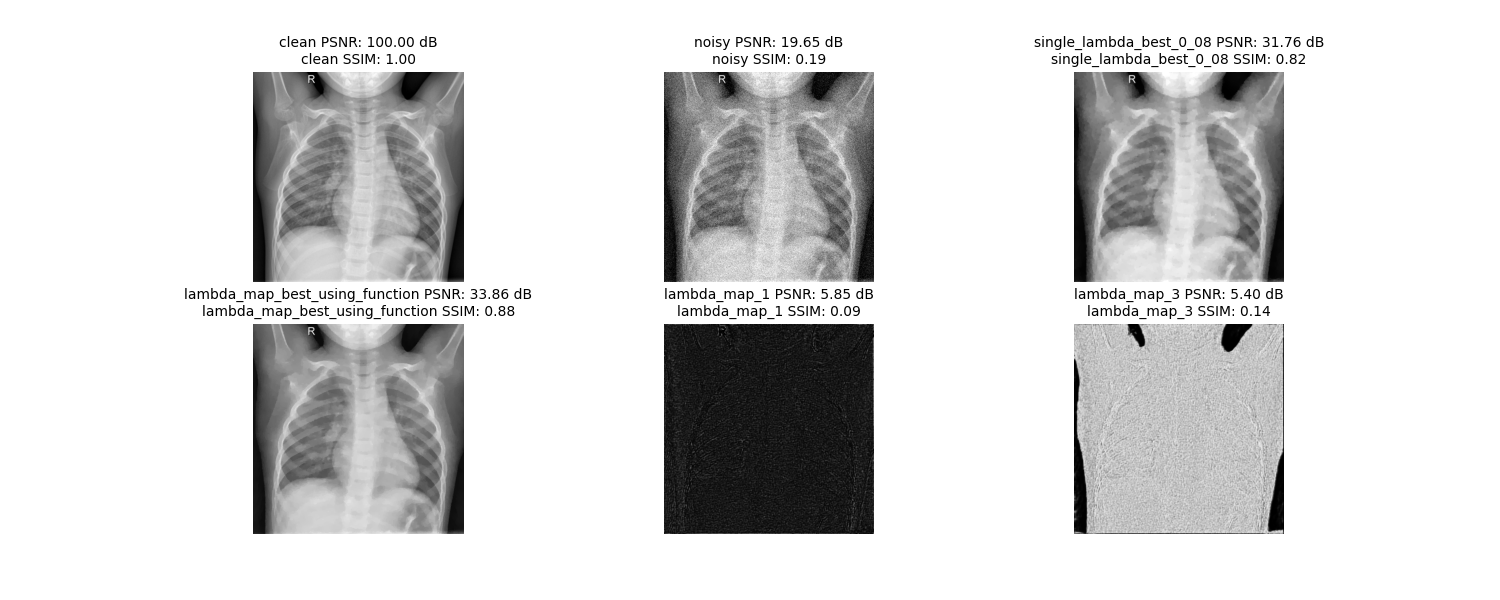
\includegraphics[width=1\linewidth]{images//chest_xray/results.png}
        
%     \caption{$512 \times 512$, $\text{T}=128$, $\sigma=0.5$, $\lambda=0.08$}
%     \label{fig:chest_xray}
% \end{figure}

% \begin{figure}[ht]
%     \centering
%     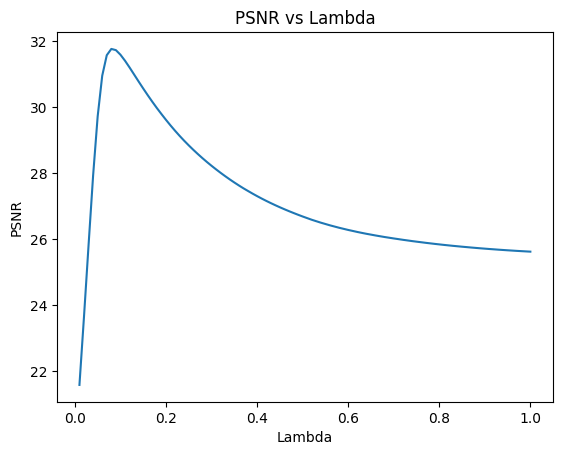
\includegraphics[width=0.6\linewidth]{images//chest_xray/Lambda vs PSNR.png}
        
%     \caption{$512 \times 512$, $\text{T}=128$, $\sigma=0.5$, $\lambda=0.08$}
%     \label{fig:chest_xray}
% \end{figure}




% \subsubsection{Part 5.5 CT experiment}

% Original dataset: 35820 images training, 3522 validation, 3553 testing

% Actually uses: 300 images training, 10 validation, no test

% 362 x 362, 300 images --> 39,313,200 pixels per epoch

% UNet 32, 64, 128 --> 610,673 trainable parameters

% 39,313,200  \times  610,673  =  2.400751e+13

% Adam optimizer with a learning rate of 10−4

% a batch size of 1

% train for 50 epochs

% Then we used the model configuration for which the MSE on the validation set was lowest. ???

% T = 512

% 39,313,200  \times  610,673  \times  512  =  1.2291845e+16 

% 24 hours

% single NVIDIA GeForce RTX 2080 super GPU with 8 GB GPU

% 1 epoch = 300 iterations, took 5 hours = 300 minutes


% --------

% Mine: 


% 32, 64, 128, 256 --> 1,796,034 trainable parameters, check using code

% 1000 training images, 256 * 256 --> total 65,536,000 pixels per epoch


% 65,536,000  \times  1,796,034  =  1.1770488e+14

% T = 256

% 65,536,000  \times  1,796,034  \times  256  =  3.013245e+16


% Adam optimizer with a learning rate of 10−4, a batch size of 1

% 1 epoch took 20 minutes


% 2.5 times more work  but  2/30  amount of time







% \section{Training and Results}

% % \subsection{Objective and Setup}

% The primary aim of this project is to explore the potential of achieving the optimal regularisation parameter map, $\mathbf{\Lambda}$, for a particular image. To this end, the training was conducted on a single image, using a grid search to determine the best single regularisation parameter, $\lambda$. The chosen $\lambda = 0.05$ yielded a PSNR (Peak Signal-to-Noise Ratio) of 35.64 dB, considered to be within the good range (30-40 dB). Our model, utilizing the regularisation map $\mathbf{\Lambda}$, improved the PSNR to 37.84 dB compared to the 24.13 dB of the noisy original, demonstrating the efficacy of the model-specific parameter map.

% \subsection{Data Preparation and Model Configuration}

% Training was performed on image ID 0065, which was rescaled by a factor of 0.5 and split into six 512$\times$512 patches. Gaussian noise (mean 0, standard deviation 0.3) was added to simulate conditions for robust model training. The model was trained with a batch size of 1, resulting in six iterations per epoch, over 10,000 epochs.

% \subsection{Training Details}

% The Mean Squared Error (MSE) loss function was chosen due to its effectiveness in Gaussian noise contexts. The Adam optimiser was utilized for its adaptive learning rate capabilities, set at 0.0001. LeakyReLU activation function with $\alpha = 0.01$ was used across all hidden layers to ensure non-linearity without significant information loss at zero activations. 

% The PDHG (Primal Dual Hybrid Gradient) solver, an integral part of the model, was run for 128 iterations per epoch. While increasing the number of iterations might improve results, time constraints limited our exploration.

% \subsection{Performance Metrics and Results}

% Performance was evaluated using the PSNR metric, calculated as:
% $$
% \text{PSNR} = 10 \cdot \log_{10} \left( \frac{{\text{MAX}^2}}{{\text{MSE}}} \right)
% $$
% where $\text{MAX}$ is the maximum possible pixel value, and $\text{MSE}$ is the mean squared error between the original and reconstructed images. 

% Each epoch of training took approximately 6 seconds, translating to about 1 second per patch. The total training duration was around 17 hours, dominated by the computational demands of the PDHG algorithm.

% \subsection{Inference and Efficiency}

% The inference time for our model was about 1 second per 512$\times$512 patch. For a full HD (1920$\times$1080) image, denoising required processing 12 patches, taking less than half a minute in total. This demonstrates that while our method is slower than traditional single-parameter denoising methods, it offers a systematic approach to optimizing regularisation without prior knowledge of the best $\lambda$.

% \begin{figure}[ht]
%     \centering
%     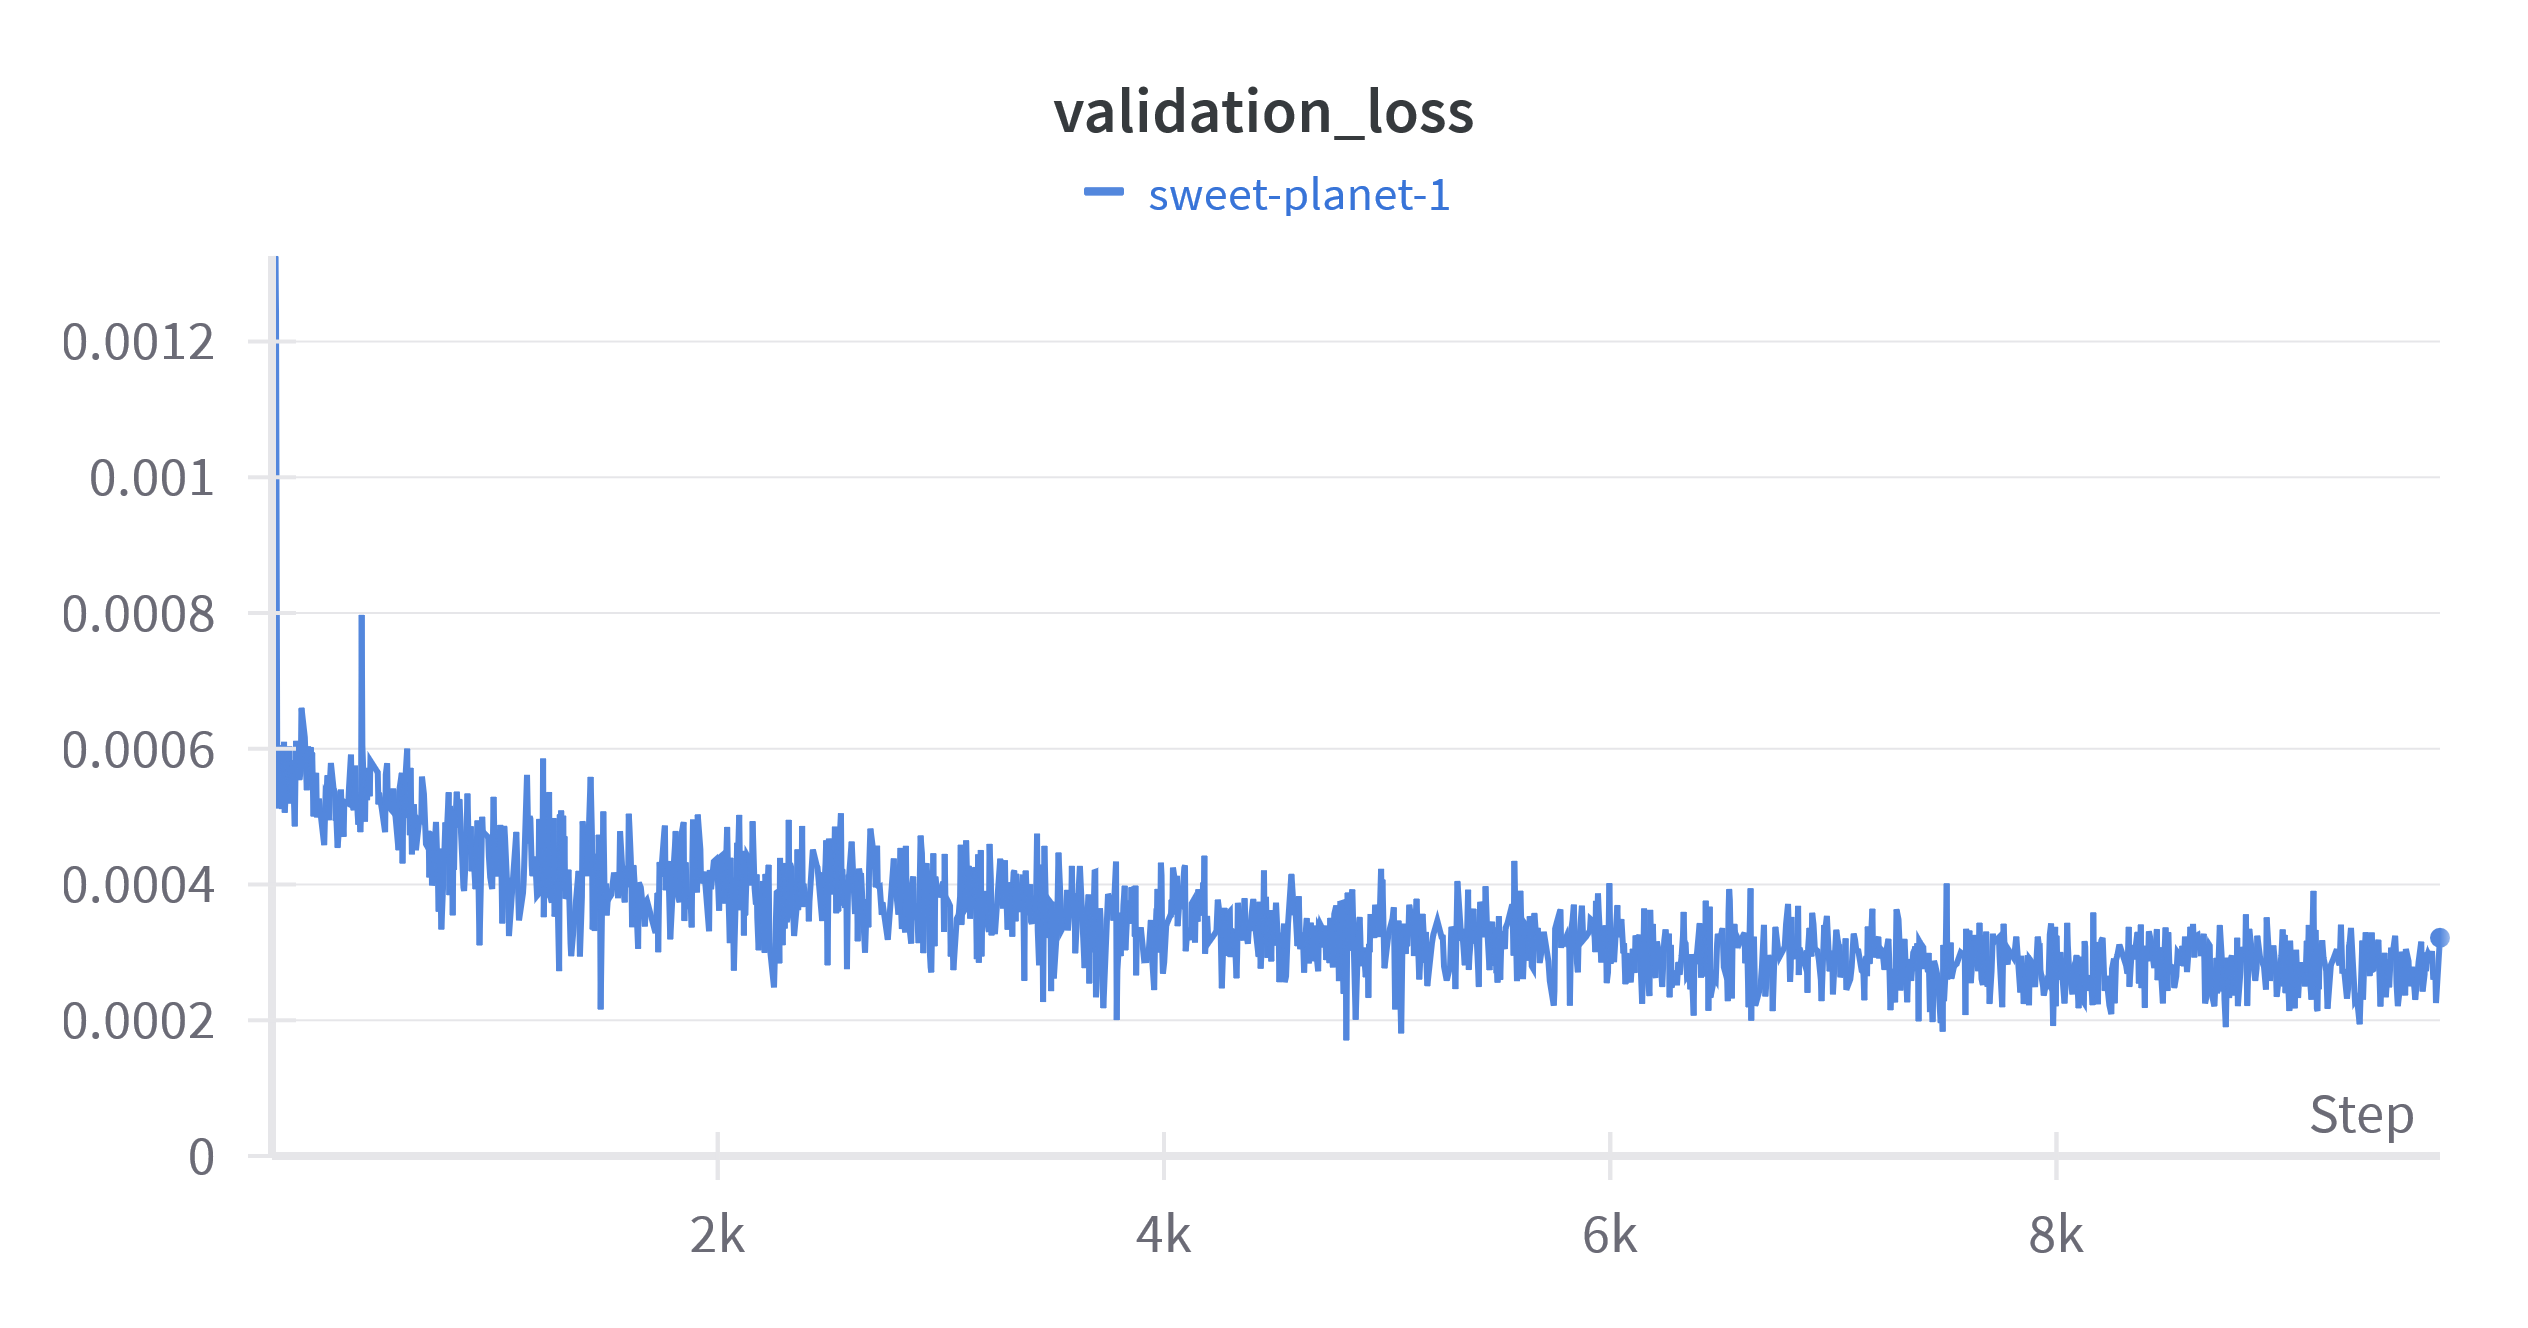
\includegraphics[width=0.6\linewidth, trim={0 0 0 10cm}, clip]{images/W&B Chart 5_27_2024, 5 09 06 PM.png}
%     \caption{Validation loss. Logged using wandb} 
%     \label{fig:training_progress}
% \end{figure}

% \begin{figure}[ht]
% % \begin{center}
% \centering
% \begin{tabular}{ c c c c c c c c c }
%  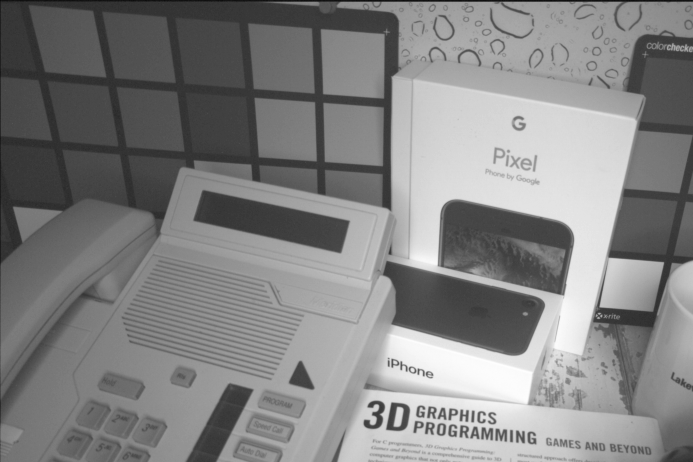
\includegraphics[width=0.4\linewidth]{images/cur/image_clean.png}  & 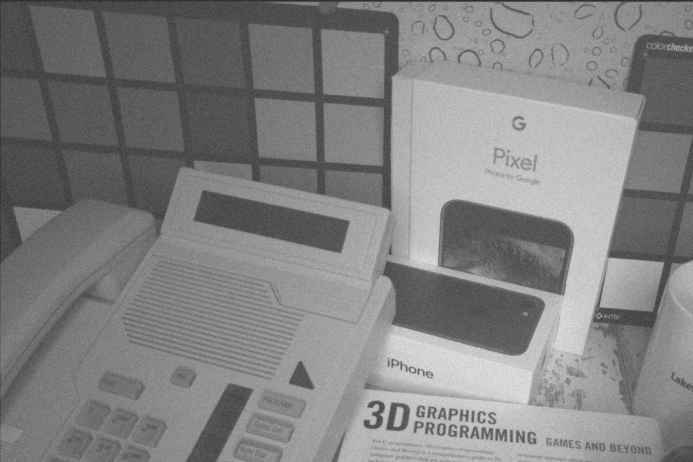
\includegraphics[width=0.4\linewidth]{images/cur/image_noisy.png} \\
%  Clean image & Noisy image. PSNR 24.13 dB \\
%    &  \\
%  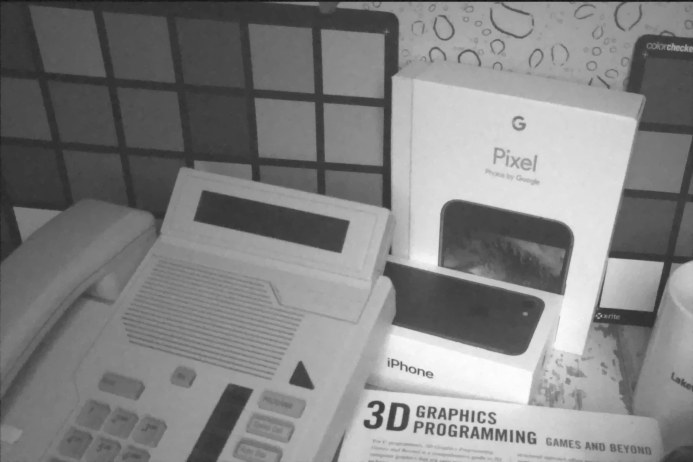
\includegraphics[width=0.4\linewidth]{images/cur/image_denoised_single_lambda.png} & 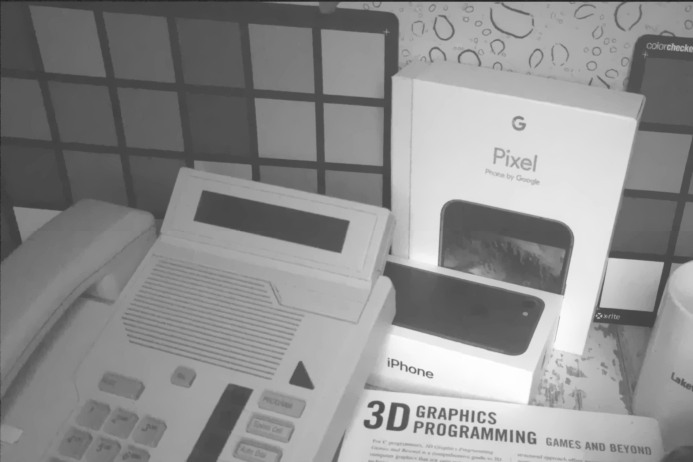
\includegraphics[width=0.4\linewidth]{images/cur/image_denoised_lambda_map.png}   \\
%  Denoised with $\lambda = 0.05$. PSNR 35.64 dB & Denoised with $\mathbf{\Lambda}$ map. PSNR 
%  \textcolor{blue}{37.84 dB}  \\

 
% \end{tabular}

%     \caption{Comparison of output using single $\lambda$ and $\mathbf{\Lambda}$ map}


% % \end{center}
% \end{figure}

% \begin{figure}[ht]
%     \centering
%     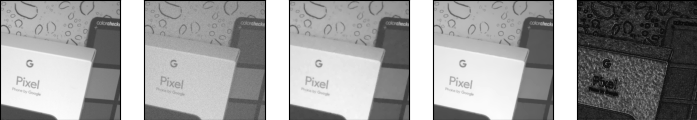
\includegraphics[width=1.0\linewidth]{images/cur/patch_2.png}
%     \vspace{-8pt}
    
%     \caption{Comparison of patches. From left to right: (1) Original image. (2) Noisy image with synthetic Gaussian noise added with $\sigma = 0.3$. (3) Reconstruction with single $\lambda = 0.03$. (4) Reconstruction with $\mathbf{\Lambda}$ map. (5) Output of the U-Net: $\mathbf{\Lambda}$ map.}
%     \label{fig:compare_patches}
% \end{figure}

% \subsection{Analysis of the $\mathbf{\Lambda}$ Map}

% The $\mathbf{\Lambda}$ map generated by our model provides a visual representation of how the PDHG solver is directed to handle different regions of the image. In areas where the original image was predominantly white, such as on a box, the $\mathbf{\Lambda}$ map exhibits higher regularisation values, indicated by whiter pixels. This implies that the PDHG solver is instructed to penalize high gradients in these regions, effectively smoothing them out.

% Conversely, areas with intricate details, such as text on the box, display lower regularisation values, represented by darker pixels on the $\mathbf{\Lambda}$ map. This indicates that the solver is tuned to preserve finer details in these areas, maintaining clarity and sharpness.

% % \subsubsection*{Challenges in regularisation}

% Despite the intended function of the regularisation map, there are instances where the model does not perform as expected. For example, the squares on the color palettes in the background, which originally had smooth surfaces, should ideally exhibit high regularisation values. However, this is not always the case, suggesting areas for further refinement in the model's ability to accurately assess and respond to different textural features within an image.


% \begin{figure}[ht]
%   \centering
%   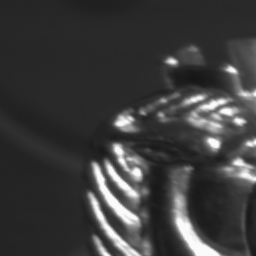
\includegraphics[width=0.34\linewidth]{100-clean.png}
%   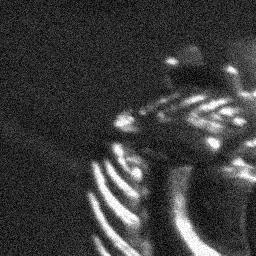
\includegraphics[width=0.34\linewidth]{100-noisy-mse.png}
%   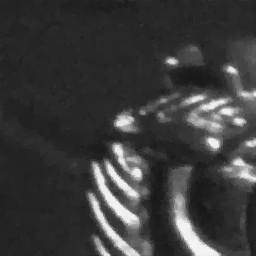
\includegraphics[width=0.34\linewidth]{100-psnr_34.02-lambda_0.04.png}
%   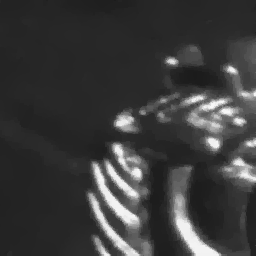
\includegraphics[width=0.34\linewidth]{100-denoised-mse_24.42-psnr_34.29-ssim_0.96.png}
%   \caption{SIDD example: Clean, Noisy, $\lambda = 0.04$ with PSNR = 34.02, $\mathbf{\Lambda}_\Theta$ with PSNR = 34.29}
%   \label{fig:SIDD-chest-example-1}
% \end{figure}


% \section{Conclusion}

% In this dissertation we have described the theory of application of total variational (TV) method to image denoising.
% We have also described the implementation of the method and an improvement using a U-Net architecture to find the regularisation parameters more efficiently.
% We have then presented the results of the method on a few different datasets.





% \begin{figure}[ht]
%     \centering
%     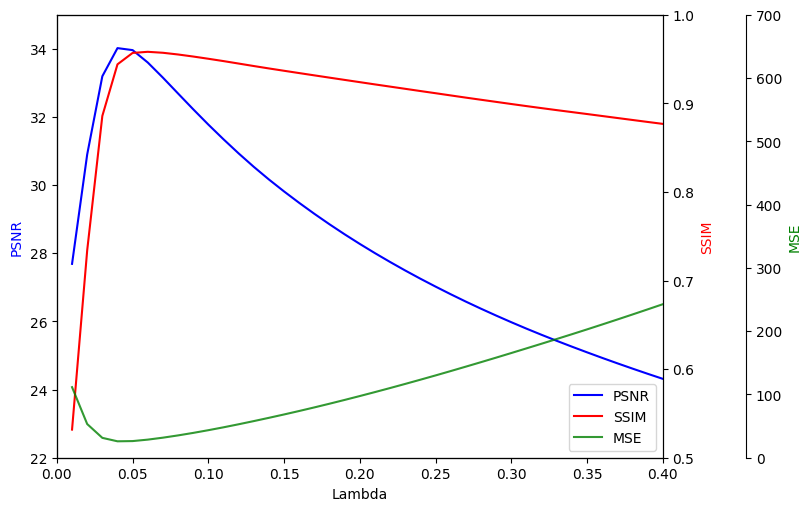
\includegraphics[width=0.8\linewidth]{100-line_plots.png}
%     \caption{SIDD example: grid search}
%     \label{fig:enter-label}
% \end{figure}




% \section{Test cases}

% \subsection{Tutle}

% \begin{figure}[ht]
%     \centering
%     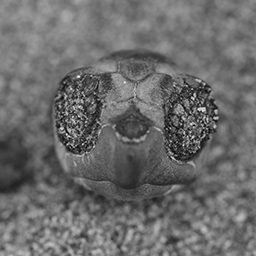
\includegraphics[width=0.25\linewidth]{images/tests/turtle clean.png}
%     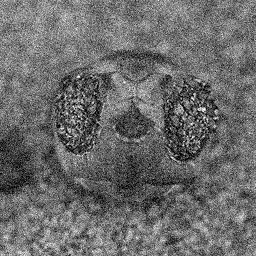
\includegraphics[width=0.25\linewidth]{images/tests/turtle noisy.png}
%     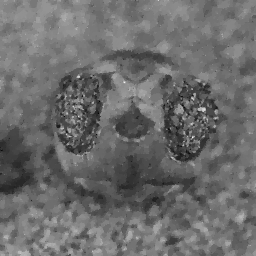
\includegraphics[width=0.25\linewidth]{images/tests/turtle single lambda.png}
%     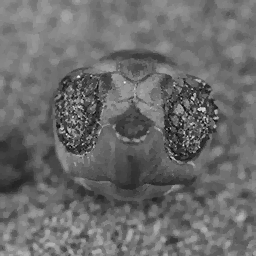
\includegraphics[width=0.25\linewidth]{images//tests/turtle_denoised_overfit.png}
%     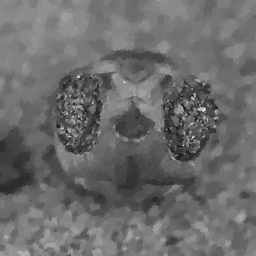
\includegraphics[width=0.25\linewidth]{images/tests/turtle lambda map.png}
%     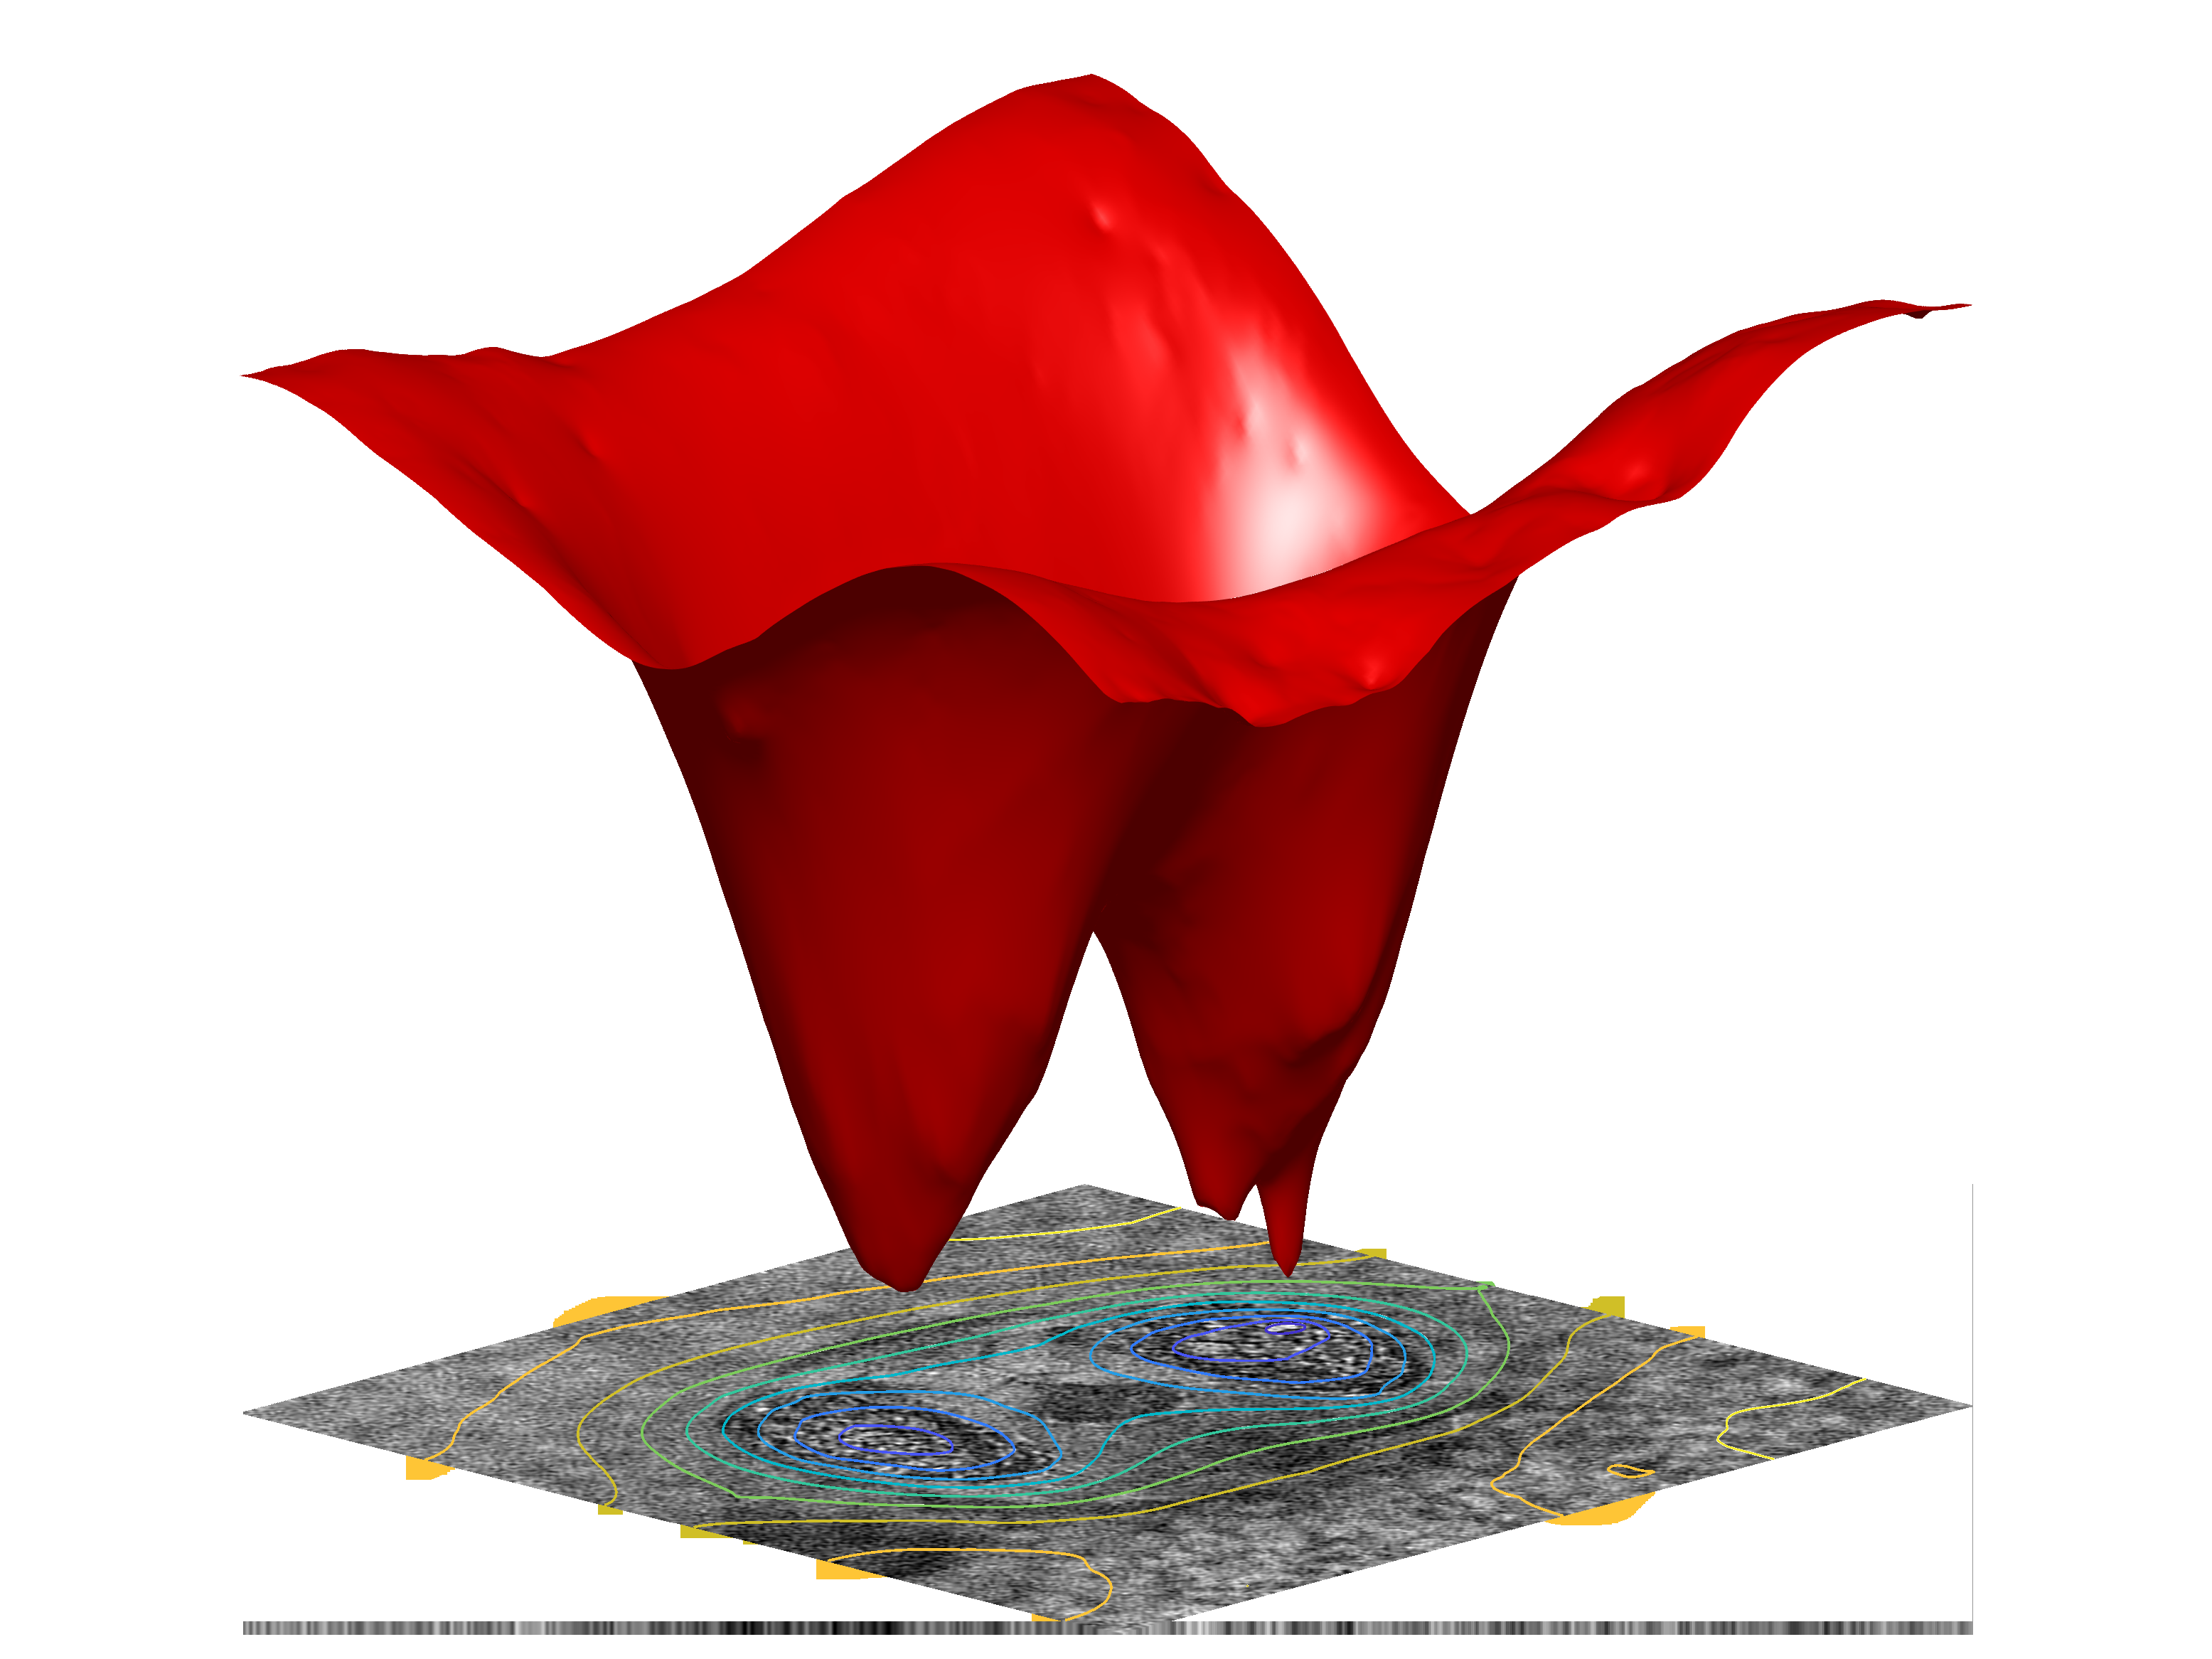
\includegraphics[width=0.25\linewidth]{images/tests/turtle lambda map graph.png}
%     \caption{turtle: clean; noisy; single $\lambda = 0.07$; lambda map $\mathbf{\Lambda}$}
%     \label{fig:enter-label}
% \end{figure}


% \subsection{Square}

% \begin{figure}[ht]
%     \centering
%     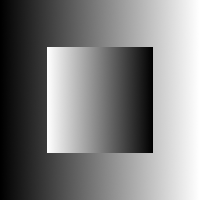
\includegraphics[width=0.19\linewidth]{images/tests/square clean.png}
%     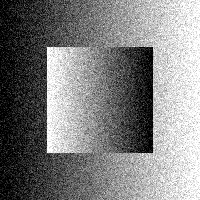
\includegraphics[width=0.19\linewidth]{images/tests/square noisy.png}
%     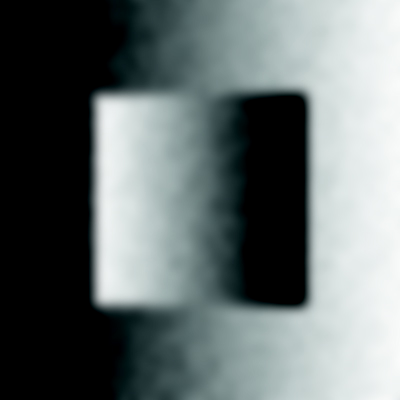
\includegraphics[width=0.19\linewidth]{images/tests/square tikhonov.png}
%     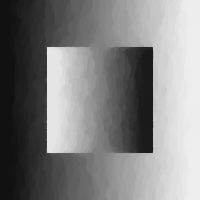
\includegraphics[width=0.19\linewidth]{images/tests/square TV single lambda.png}
%     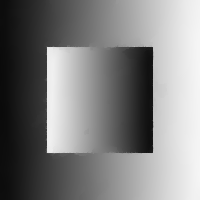
\includegraphics[width=0.19\linewidth]{images/tests/square TGV single lambdas.png}
%     \caption{square: clean; noisy; Tikhonov; TV single $\lambda$; TGV single $\lambda_1$ and $\lambda_2$}
%     \label{fig:square_clean}
% \end{figure}




% \section{Data}



% \url{https://openaccess.thecvf.com/content_CVPRW_2019/papers/NTIRE/Abdelhamed_NTIRE_2019_Challenge_on_Real_Image_Denoising_Methods_and_Results_CVPRW_2019_paper.pdf}

% Gaussian $\sigma$, the estimated range is [0.242, 11.507]
% in the space of [0, 255].

% The validation data consisted of 1280 noisy image blocks
% (i.e., croppings) form both raw-RGB and sRGB images,
% each block is 256×256 pixels. The blocks are taken from 40
% images, 32 blocks from each image (40 × 32 = 1280). All
% image blocks are combined in a single 4D array of shape
% [40, 32, 256, 256] where the four dimensions represent the
% image index, the index of the block within the image, the
% block height, and the block width, respectively. The blocks
% have the same number format as the training data. 

% The testing data consisted of 1280 noisy image blocks different from the validation block but following the same format
% as the validation data. Image metadata files were also provided for the 40 images from which the validation/testing
% data was extracted.





% \subsubsection{Other experiment B (ruby-dust-28)}:

% \url{https://wandb.ai/wof/chest_xray/runs/0ntx5gs4}

% \begin{minted}[frame=single,
%                framesep=3mm,
%                linenos=true,
%                xleftmargin=21pt,
%                fontsize=\small,
%                tabsize=4]{Json}

% {
%   "T": {
%     "value": 32
%   },
%   "epochs": {
%     "value": 10000
%   },
%   "dataset": {
%     "value": "../data/chest_xray"
%   },
%   "project": {
%     "value": "chest_xray"
%   },
%   "n_blocks": {
%     "value": 3
%   },
%   "up_bound": {
%     "value": 0
%   },
%   "max_sigma": {
%     "value": 0.5
%   },
%   "min_sigma": {
%     "desc": null,
%     "value": 0.5
%   },
%   "optimizer": {
%     "desc": null,
%     "value": "Adam"
%   },
%   "activation": {
%     "desc": null,
%     "value": "LeakyReLU"
%   },
%   "batch_size": {
%     "desc": null,
%     "value": 1
%   },
%   "wandb_mode": {
%     "desc": null,
%     "value": "online"
%   },
%   "in_channels": {
%     "desc": null,
%     "value": 1
%   },
%   "random_seed": {
%     "desc": null,
%     "value": 42
%   },
%   "architecture": {
%     "desc": null,
%     "value": "UNET-PDHG"
%   },
%   "init_filters": {
%     "desc": null,
%     "value": 32
%   },
%   "out_channels": {
%     "desc": null,
%     "value": 2
%   },
%   "learning_rate": {
%     "desc": null,
%     "value": 0.0001
%   },
%   "loss_function": {
%     "desc": null,
%     "value": "MSELoss"
%   },
%   "resize_square": {
%     "desc": null,
%     "value": 256
%   },
%   "val_data_path": {
%     "desc": null,
%     "value": "../data/chest_xray/val/NORMAL"
%   },
%   "test_data_path": {
%     "desc": null,
%     "value": "../data/chest_xray/test/NORMAL"
%   },
%   "train_data_path": {
%     "desc": null,
%     "value": "../data/chest_xray/train/NORMAL"
%   },
%   "upsampling_mode": {
%     "desc": null,
%     "value": "linear_interpolation"
%   },
%   "val_num_samples": {
%     "desc": null,
%     "value": 8
%   },
%   "save_epoch_local": {
%     "desc": null,
%     "value": 10
%   },
%   "save_epoch_wandb": {
%     "desc": null,
%     "value": 10000
%   },
%   "test_num_samples": {
%     "desc": null,
%     "value": 1
%   },
%   "downsampling_mode": {
%     "desc": null,
%     "value": "max"
%   },
%   "train_num_samples": {
%     "desc": null,
%     "value": 100
%   },
%   "upsampling_kernel": {
%     "desc": null,
%     "value": [
%       2,
%       2,
%       1
%     ]
%   },
%   "downsampling_kernel": {
%     "desc": null,
%     "value": [
%       2,
%       2,
%       1
%     ]
%   }
% }

% \end{minted}






% \subsection{MRI}

% \begin{figure}[ht]
%     \centering
%     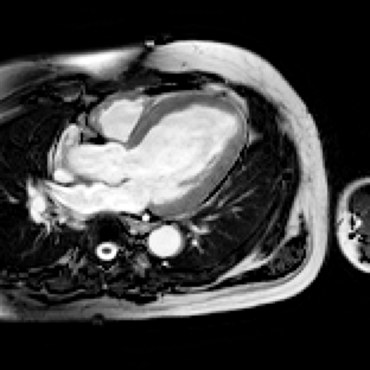
\includegraphics[width=0.25\linewidth]{images//tests/MRI.png}
%     \caption{Enter Caption}
%     \label{fig:enter-label}
% \end{figure}




\section{Results}
% Each test image was also noised with Gaussian noise with a random value of $\sigma$ ranging from 0.1 to 0.5.

As previously mentioned, we used 100 images with label "normal" from the test set provided in the Chest X-ray dataset for testing.
Each test image was noised with a Gaussian noise of mean 0 and standard deviation $\sigma = 0.5$.
For each test image, we also did a grid search with 81 equally spaced values between 0 and 0.8 in order to find the best scalar $\lambda$ for the total variational denoising method, which we used as a baseline to show the effectiveness of our method.

% We compare the results using the regularisation parameter map generated by
% our method with the results using a scalar $\lambda$ for the total variational denoising method.
% For each test image, we run a grid search to find the best scalar $\lambda$.

As an example, we present the results for one of the test images.
The results of the grid search is shown in the line plots in figure 4.
For this particular test image, the highest value of PSNR of 29.945 dB was achieved by $\lambda = 0.07$.
The regularisation parameter map $\mathbf{\Lambda}_\Theta$ found using $\text{NET}_{\Theta}$ resulted in a PSNR of 31.248 dB.
The clean and orignal versions as well as the resulting denoised images are shown in Figure 5.

\begin{figure}[H]
  \centering
  % 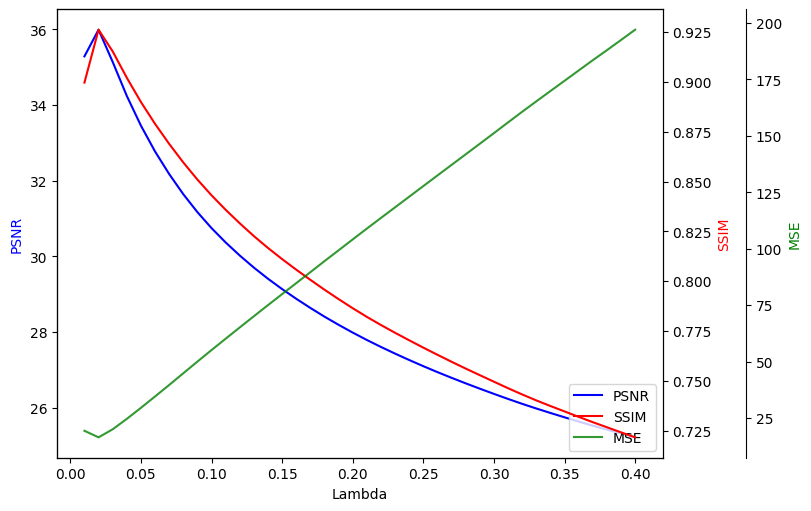
\includegraphics[width=0.6\linewidth]{images//chest_xray/chest_xray-line_plots.png}
  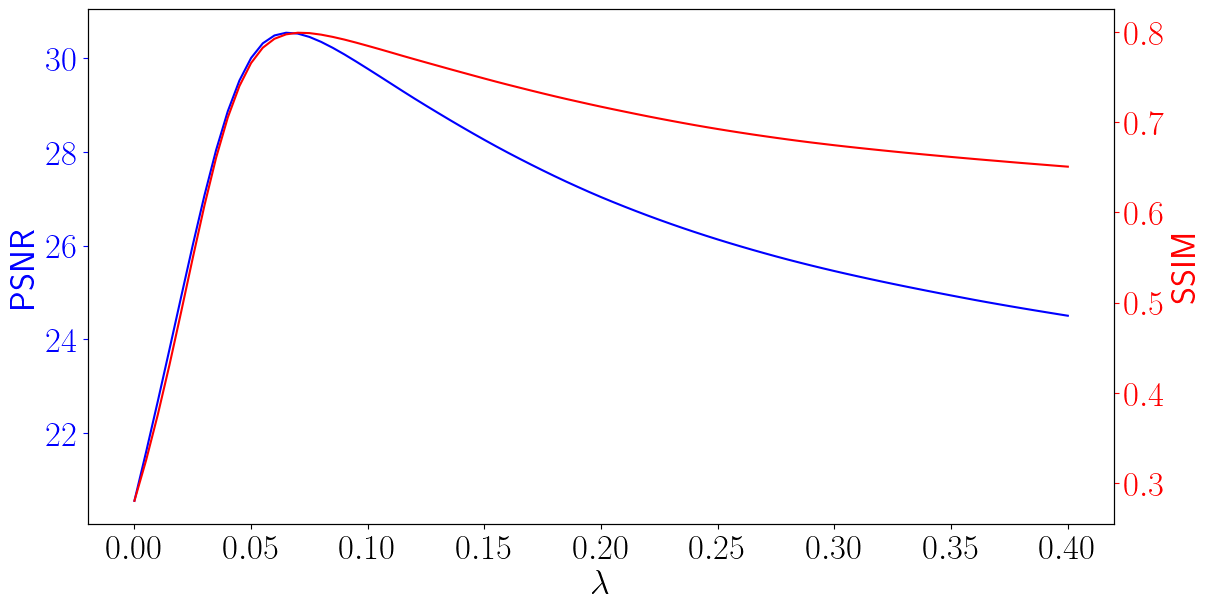
\includegraphics[width=0.66\linewidth]{images//chest_xray/ex_2/pyplot_multiple_y-axis.PNG}
  
      \caption{Grid search for the best scalar regularisation parameter $\lambda$ for the example test image. The highest PSNR of 29.945 dB was achieved by $\lambda = 0.07$.}
  \label{fig:line_plots}
\end{figure}

% \begin{figure}[ht]
%   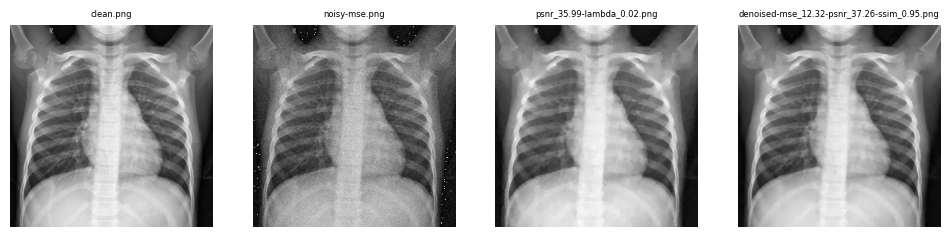
\includegraphics[width=1\linewidth]{images//chest_xray/chest_xray-denoised_compare.png}
%   \caption{Chest X-ray example - denoised images}
%   \label{fig:chest_xray}
% \end{figure}



% \begin{figure}[ht]
%   \centering
  
%   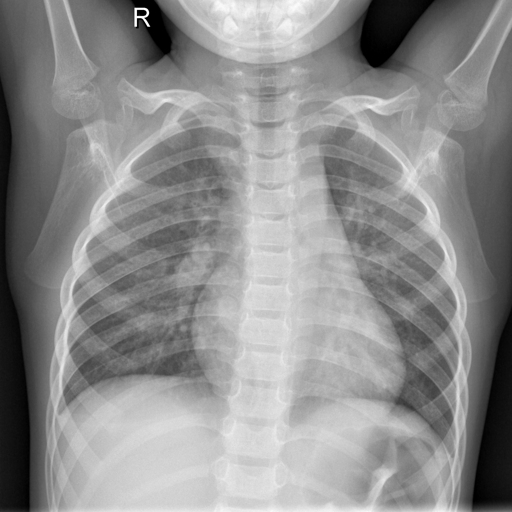
\includegraphics[width=0.25\linewidth]{images//chest_xray/clean.png}
%   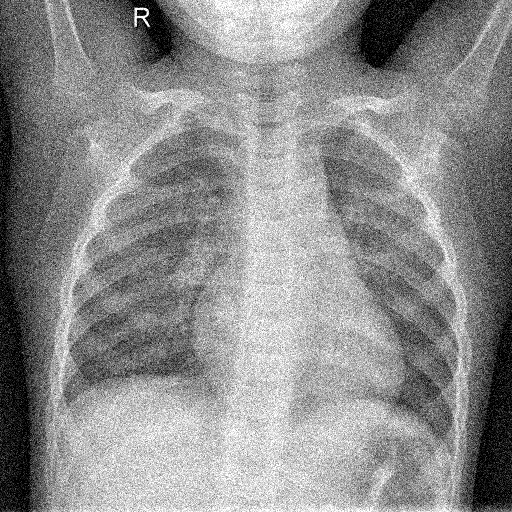
\includegraphics[width=0.25\linewidth]{images//chest_xray/noisy.png}
%   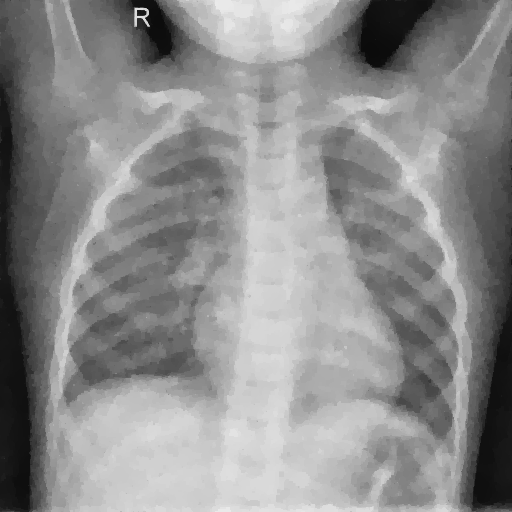
\includegraphics[width=0.25\linewidth]{images//chest_xray/single_lambda_best_0_08.png}
%   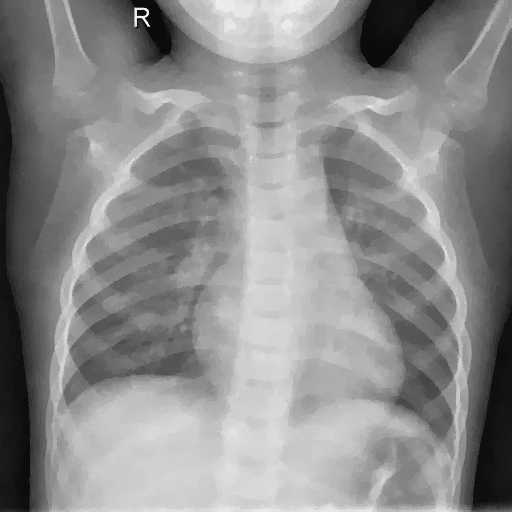
\includegraphics[width=0.25\linewidth]{images/chest_xray/lambda_map_best_using_function.png}
%   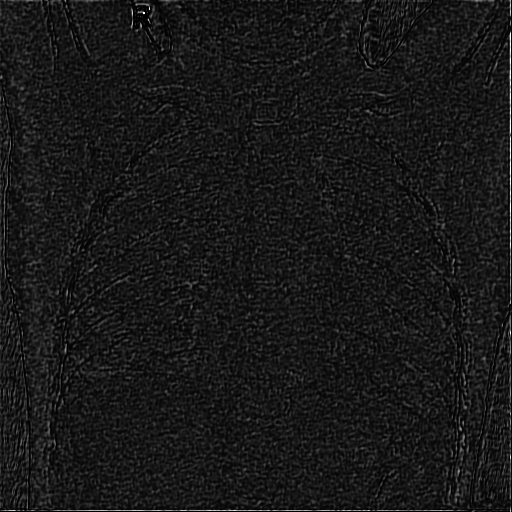
\includegraphics[width=0.25\linewidth]{images//chest_xray/lambda_map_1.png}
%   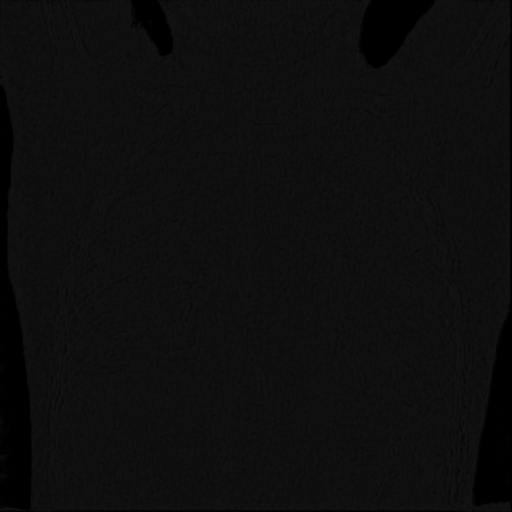
\includegraphics[width=0.25\linewidth]{images//chest_xray/lambda_map_3.png}
      
%   % \caption{$512 \times 512$, $\text{T}=128$, $\sigma=0.5$, $\lambda=0.08$}
%   \caption{Chest X-ray example: clean, noisy, denoised using scalar $\lambda = 0.02$ with PSNR = 35.99, denoised using $\mathbf{\Lambda}_\Theta$ with PSNR = 37.26, $\mathbf{\Lambda}_\Theta$}
%   \label{fig:chest_xray}
% \end{figure}



% \begin{figure}[ht]
%   \centering
%   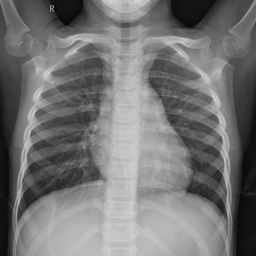
\includegraphics[width=0.34\linewidth]{images//chest_xray/100-clean.png}
%   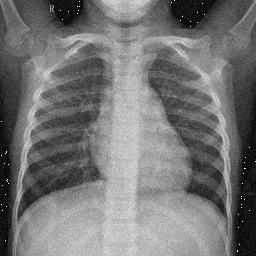
\includegraphics[width=0.34\linewidth]{images//chest_xray/100-noisy.png}
%   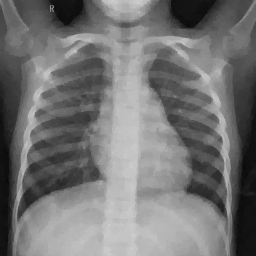
\includegraphics[width=0.34\linewidth]{images//chest_xray/100-psnr_35.99-lambda_0.02.png}
%   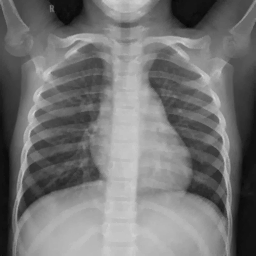
\includegraphics[width=0.34\linewidth]{images//chest_xray/100-lambda_map-psnr_37.26-ssim_0.95.png}
%   \caption{Chest X-ray example: clean, noisy, $\lambda = 0.02$ with PSNR = 35.99, $\mathbf{\Lambda}_\Theta$ with PSNR = 37.62}
%   \label{fig:enter-label}
% \end{figure}

% \newpage

\begin{figure}[ht]
  \centering
  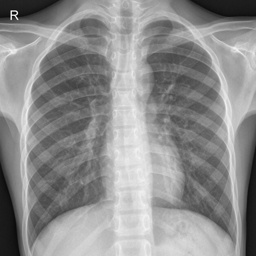
\includegraphics[width=0.34\linewidth]{images//chest_xray/ex_2/clean.png}
  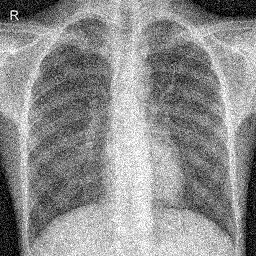
\includegraphics[width=0.34\linewidth]{images//chest_xray/ex_2/noisy.png}
  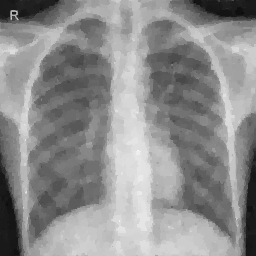
\includegraphics[width=0.34\linewidth]{images//chest_xray/ex_2/psnr_29.945-lambda_0.07.png}
  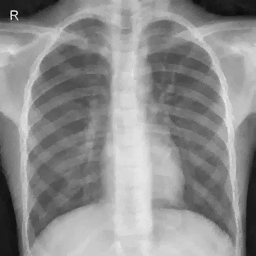
\includegraphics[width=0.34\linewidth]{images//chest_xray/ex_2/denoised-mse_49.17-psnr_31.248-ssim_0.831.png}
  \caption{Chest X-ray example. The top row shows the original image on the left and the noisy image, generated with Gaussian noise with $\sigma = 0.5$. The bottom row shows the denoised images using the TV method; the left image with PSNR = 29.945 was produced using the best scalar regularisation parameter $\lambda = 0.07$ , while the right image with PSNR = \textbf{31.248} was denoised using the regularisation parameter map $\mathbf{\Lambda}_\Theta$ found using $\text{NET}_\Theta$.}
  \label{fig:enter-label}
\end{figure}


\newpage



% \begin{wrapfigure}{l}{1\textwidth}
\begin{figure}[ht]
  \centering
  \begin{subfigure}{0.48\textwidth}
  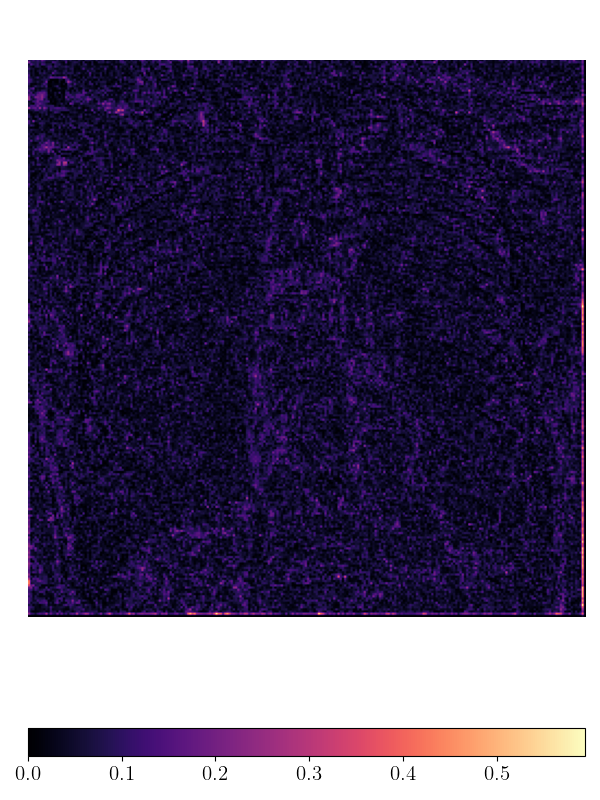
\includegraphics[width=1\linewidth]{images//chest_xray/ex_2/lambda_map.png}
  \includegraphics[width=1\linewidth]{images//chest_xray/ex_2/lambda_map_values_histogram.png}\
  \caption{$\mathbf{\Lambda}_{\Theta}$ map and histogram of the values}
  \end{subfigure}
  \begin{subfigure}{0.48\textwidth}
  \includegraphics[width=1\linewidth]{images//chest_xray/ex_2/lambda_map_log.png}
  \includegraphics[width=1\linewidth]{images//chest_xray/ex_2/lambda_map_values_histogram_log.png}
  \caption{$\log{(\mathbf{\Lambda}_{\Theta} + 0.05)}$ and histogram of the log values}
  \end{subfigure}
  \caption{The produced $\mathbf{\Lambda}_{\Theta}$ map for the chest x-ray dataset example. Since the values are too close to one another in the lower spectrum, the bottom row shows the log of the map and the histogram of the log values for better separation.}
  \label{fig:enter-label}
\end{figure}
% \end{wrapfigure}{l}

Qualitatively, we can see that there is a good reduction in the stair-case effect in the denoised image using the regularisation parameter map $\mathbf{\Lambda}_\Theta$ compared to the denoised image using the scalar $\lambda$.

\newpage







% \begin{figure}[ht]
%   \centering
%       \includegraphics[width=1\linewidth]{images//chest_xray/outputa.png}
%       \caption{Chest X-ray box plots}
%   \label{fig:enter-label}
% \end{figure}

\begin{figure}[ht]
  \centering
  % \includegraphics[width=1\linewidth]{images//chest_xray/output3.png}
  \includegraphics[width=0.5\linewidth]{images//chest_xray/box_plots_1.png}
  \caption{Test results summary}
  \label{fig:box_plots}
\end{figure}

% \documentclass{article}
% \usepackage{amsmath}
% \usepackage{graphicx}

\begin{table}[h!]

\centering
\begin{tabular}{c|c c}
% \hline
 & \textbf{PDHG -} $\lambda$ & \textbf{PDHG -} $\mathbf{\Lambda}_{\Theta}$ \\
\hline
\textbf{SSIM} & $0.87 \pm 0.04$ & $\mathbf{0.90} \pm 0.03$ \\
\textbf{PSNR} & $33.43 \pm 2.16$ & $\mathbf{34.73} \pm 2.02$ \\
% \hline
\end{tabular}

\caption{Mean and standard deviation of the measures SSIM and PSNR obtained over the test set for the chest x-ray dataset example. 
The TV-reconstruction using the parameter-map $\mathbf{\Lambda}_{\Theta}$ improves both measures.
}

\label{table:1}

\end{table}

\begin{figure}[H]
  \centering
  \includegraphics[width=0.48\linewidth]{images//chest_xray/hist_psnr_diff.png}
  \includegraphics[width=0.48\linewidth]{images//chest_xray/hist_ssim_diff.png}
  \caption{Histograms of the PSNR and SSIM differences between using $\lambda$ scalar and using $\mathbf{\Lambda}_{\Theta}$ map for
  reconstructions of noisy versions of the test images. 
  The $\mathbf{\Lambda}_{\Theta}$ map method consistently outperforms the scalar $\lambda$ method.
  % In all bilevel algorithms the
  % ground truth-free statistics-based upper level objective was used.
  }
  \label{fig:hist_diff}
\end{figure}

Plotting the values for all the test images, we can see that the regularisation parameter map consistently outperforms the scalar $\lambda$.
The box plots in Figure \ref{fig:box_plots} show the distribution of PSNR and SSIM values for the test images
using the two methods.
The regularisation parameter map consistently produces higher PSNR and SSIM values than the scalar $\lambda$.

% More visualisations:

% - Histograms of the PSNR and SSIM differences (see Figure 9 of Dualization paper)

% - Show Lambda map: use a different colormap with legend showing the range of the values (0.00 to 0.05) (page 29 of the paper)

% - Table of PSNR and SSIM values for each image: Table 4 in paper

% - Scale the box plots like figure 13 in paper

- (More experiments) Test with the sigma 0.1 and 0.3 for test images and add: box plots, table rows, and difference histograms.




% The total variational denoising method was able to produce denoised images that were closer to the ground truth images.


\section{Conclusion}



This project showcases the integration of neural networks with traditional algorithms to enhance image denoising capabilities, marking a significant step forward in computational imaging.

\subsection{Experimentation and Findings}

We experimented with the capabilities of the U-Net architecture to learn and apply regularisation parameters dynamically across different image segments using the PDHG algorithm. Traditional denoising techniques typically rely on a single lambda value for regularisation, which often does not cater to the varying needs across an image. Our approach attempts to transcend this limitation by approximating an optimal lambda map through the U-Net, enhancing the PDHG's performance. This methodology, while computationally intensive, illustrates the potential benefits of segment-specific regularisation in image denoising.

% \subsection{Real-World Implications and Limitations}

% Because of the considerable computation time, this limited our ability to extend the experiment across different sets of images. 
% Moving forward, optimizing the computational efficiency of this model will be crucial for broader application and scalability.

% \subsection{Conclusion}
In conclusion, while the experiment demonstrated potential improvements over traditional single-lambda denoising methods, the current computational demands make it impractical for real-world applications. 

\section{Future Work}

% Future research will focus on refining the efficiency of these neural network-enhanced denoising techniques to make them more viable for practical use.


\newpage




\printbibliography


The following list contain the primary Python libraries used in the implementation of this project.

\vspace{-6pt}

\begin{itemize}
\setlength\itemsep{-0.3em}
  \item \codeword{NumPy}: Utilised for numerical representations and operations, including vector and matrix multiplication.
  \item \codeword{PyTorch}: Employed for constructing and training neural network models due to its robust, flexible, and efficient computational dynamics.
  \item \codeword{matplotlib} and \codeword{seaborn}: Employed for data visualisation tasks, including the creation of histograms, box plots, and other graphical representations.
  % \item \codeword{pandas}: Used for data analysis and manipulation tasks, such as managing data frames and handling value replacement operations.
  \item \codeword{scikit-learn}: Used for benchmarking our model against traditional machine learning algorithms, providing tools for data preprocessing, cross-validation, and more.
  \item \codeword{random}: Critical for generating random numbers, used extensively in stochastic processes like K-fold cross-validation and bootstrap sampling.
  \item \codeword{wandb}: Integrated for experiment tracking and logging, facilitating the monitoring of model training metrics and performance in real-time.
\end{itemize}


\end{document}
